
%%%
%%% CHAPTER
%%%
\chapter{First Law of Thermodynamics}\label{Chapter:FirstLaw}

   \begin{LearningObjectivesBlock}{Learning Objectives}
      Upon completion of this chapter, you will be able to
        \begin{enumerate}
           \item Demonstrate understanding of key concepts of energy and the first law of thermodynamics;
           \item Apply the first law of thermodynamics to assess heat transfer and power cycles;
           \item Conduct energy analysis of thermodynamic systems;
           \item Employ energy and mass balances into thermodynamic systems to assess efficiency, and correctly observe sign conventions for work and heat transfer.
        \end{enumerate}
\medskip
     Recommended reading: Chapters 2 of \citet{Atkins_Book,SmithVanNess_Book,Moran_Book} or 3 of \citet{Borgnakke_Book}.
   \end{LearningObjectivesBlock}

%%%%%%%%%%%%%%%%%%%%%%%%%%%%%%%%%%%%%%%%%%%%%%%%%%%%%%%%%%%%%%%%%
\begin{comment}
   \begin{LearningObjectivesBlock}{Learning Objectives}
      Upon completion of this chapter, you will be able to
        \begin{enumerate}
           \item {\bf Knowledge:} Define, Name, Select, State 
           \item {\bf Comprehension:} Describe, Identify, Discuss
           \item {\bf Application:} Apply, Demonstrate, Employ, Sketch
           \item {\bf Analysis:} Analyse, Compare, Calculate, Solve
           \item {\bf Synthesis:} Determine, Formulate
           \item {\bf Evaluation:} Assess, Check, Estimate, Compare, Measure, Monitor
        \end{enumerate}
\end{comment}
%%%%%%%%%%%%%%%%%%%%%%%%%%%%%%%%%%%%%%%%%%%%%%%%%%%%%%%%%%%%%%%%%

%%%% ETOC
\localtableofcontents
   
%%%
%%% SECTION
%%%
     \section{Introduction}\label{Chapter:FirstLaw:Section:Intro}\index{Work}\index{Heat}\index{Energy}
     In Section~\ref{Chapter:Introduction:Section:ThermodAnalysis}, the main elements in the thermodynamic analysis were introduced, namely {\bf open, closed and isolated systems}, {\bf surroundings} and {\bf boundaries}. The concept of {\bf energy}, {\bf work} and {\bf heat}, pivotal entities in the study of thermodynamics systems, were also defined as,
     \begin{itemize}
        \item {\bf Work} is motion against an opposing force (Eqn.~\ref{Chpt01_Work1});
        \item {\bf Energy} of a system is its capacity to produce work, and; 
        \item {\bf Heat} is the transfer of energy across boundaries caused by temperature gradient \citep{Devoe_Book}.
     \end{itemize}
     These definitions are based on observations of systems in a macro-scale, and are critical for mass and energy balances necessary for this chapter. 

%%%
%%% SECTION
%%%
     \section{The Internal Energy}\label{Chapter:FirstLaw:Section:ThermalEnergy}\index{Internal Energy}\index{Energy!Internal|see{Internal Energy}}
     \begin{subequations}
        A system, with a prescribed amount of mass, contains energy in the form of {\bf internal energy} ($U$, inherent in the internal structure), kinetic energy (linked to the motion) and potential energy (associated with external forces acting upon the mass). The total energy, $E$, associated to the system can then be expressed as 
        \begin{displaymath}
            E = \text{Internal} + \text{Kinetic} + \text{Potential} = U + E_{\text{K}} + E_{\text{P}},
        \end{displaymath}
        and the specific energy, $e$, becomes
        \begin{equation}
            e = \frc{E}{m} = u + e_{\text{K}} + e_{\text{P}} = u + \frc{1}{2}v^{2} + gz,\label{Chapter:FirstLaw:Eqn:TotalEnergy1}
        \end{equation}
        where the kinetic energy\footnote{Kinetic energy has three components: vibrational (due to the energy associated with vibration of the body), rotational (associated with the rotation motion) and translational (associated with the motion from one spatial coordinate to another).} is assumed to be due to the translational motion (thus vibrational and rotational motion are neglected) and the potential energy to be due to the constant gravitational force. In Eqn.~\ref{Chapter:FirstLaw:Eqn:TotalEnergy1}, $u$, $e_{\text{K}}$ and $e_{\text{P}}$ are specific internal, kinetic and potential energies, respectively. Kinetic and potential energies are associated with the physical state and spatial coordinates of the system, and are commonly named {\it mechanical energy}\index{Energy!Mechanical}.  The internal energy is a characteristic of the thermodynamic state of the mass and is often labelled as {\it thermal energy}\index{Energy!Thermal}.
      
       \begin{shaded}
          The internal energy is a {\it state function}, \ie its value depends only on the current state of the system and is independent of processes undertook by the system. In other words, it is a function of the properties that determine the current state of the system.
       \end{shaded}

       Let's consider a {\it control volume} with a prescribed mass; an {\it energy balance} can be performed over this control volume assuming that energy can not be either created or destroyed but just transformed. Thus, any change in energy must be due to the transfer of energy into or out of the control volume, which can be represented as work ($W$) or heat ($Q$) transfers,
      \begin{equation}
        \frc{d\mfr[E]{}{\text{cv}}}{dt} = \mfr[\dot{E}]{}{\text{cv}} = \dot{Q} + \dot{W},\label{Chapter:FirstLaw:Eqn:TotalEnergy2}
      \end{equation}
      where the {\it dot} symbol $\left(\mathbf{\dot{ }}\right)$ over the variables represents the rate of change, \ie
      \begin{displaymath}
        \left(^{\mathbf{\cdot}}\right) =\frc{d\left[^{\mathbf{\cdot}}\right]}{dt}.
      \end{displaymath}
      Equation~\ref{Chapter:FirstLaw:Eqn:TotalEnergy2} represents the rate of change (\ie {\it instantaneous rate}) of the total energy stored in the control volume, where part of the system's energy can be transferred from or into the surroundings of the control volume. In most cases, we are interested in finite changes of properties from the beginning of the process to its end, rather than instantaneous rate evaluations. In such cases, we just need to integrate the energy equation (Eqn.~\ref{Chapter:FirstLaw:Eqn:TotalEnergy1}) \wrt time, \ie from time $t_{1}$ to $t_{2}$, then after multiplying it by $dt$,
      \begin{equation}
        \mfr[dE]{}{\text{cv}} = dU + dE_{\text{K}} + d E_{\text{P}} = \delta Q + \delta W,\label{Chapter:FirstLaw:Eqn:TotalEnergy3}\footnote{Here, it is important to differentiate three mathematical symbols commonly used in thermodynamics: $d$, $\partial$ and $\delta$. $d$ and $\partial$ represent {\it exact (or total)} (Appendix~\ref{Appendix_Calculus:TotalDifferential}) and {\it partial} (Appendix~\ref{Appendix_Calculus:PartialDifferential}) differentials, respectively. $\delta$ is often used in thermodynamics study to represent {\it inexact differential} for heat and work as these variables are path-dependent.}
      \end{equation}
      we can integrate it from {\it state 1} $\left(\text{\ie at time }t_{1}\right)$ to {\it state 2} as,
      \begin{displaymath}
        \text{\bf Left-hand side: } \int\limits_{\mfr[E]{1}{\text{cv}}}^{\mfr[E]{2}{cv}}d\mfr[E]{}{\text{cv}} = \mfr[E]{t_{2}}{\text{cv}} - \mfr[E]{t_{1}}{\text{cv}} = \mfr[E]{2}{\text{cv}} - \mfr[E]{1}{\text{cv}},
      \end{displaymath}
      \begin{displaymath}
        \text{\bf Right-hand side: } \int\limits_{t_{1}}^{t_{2}} \left|\dot{Q} + \dot{W}\right|dt = \int\limits_{\text{path}}\delta Q +  \int\limits_{\text{path}}\delta W = Q_{1-2} + W_{1-2},
      \end{displaymath}
      leading to
      \begin{equation}
          \mfr[E]{2}{\text{cv}} - \mfr[E]{1}{\text{cv}} = \left[U_{2}-U_{1}\right] + \left[\frc{1}{2}m\left(v_{2}^{2}-v_{1}^{2}\right)\right] + \left[m g \left(z_{2}-z_{1}\right)\right] = Q_{1-2} + W_{1-2}.\label{Chapter:FirstLaw:Eqn:TotalEnergy3}
      \end{equation}
      Equation~\ref{Chapter:FirstLaw:Eqn:TotalEnergy3} describes the energy balance of a system with the surroundings, where the state functions (here represented by the total, internal, kinetic and potential energies) are path-independent, whereas {\bf changes in heat and work depend on the path used in the process}. 

     \end{subequations}

%%%
%%% SECTION
%%%
     \section{Exact and Inexact Differentials}\label{Chapter:FirstLaw:Section:ExactInexactDiff}\index{Exact differential}
         In Chapter~\ref{Chapter:Introduction}, we briefly defined {\it state functions}\index{State function} as thermodynamic properties that are independent of the process. For example, when water is boiled isobarically from 15$^{\circ}$C to 100$^{\circ}$C, there are infinite ways in which boiling can progress, \eg intense heat in the first 5 mins and a moderate one afterwards 'till boiling or continuous moderate heating, etc. The rate of change of the internal energy is calculated based {\bf only} on the initial and final states. The way in which the heating of water is conducted does not affect the calculation of $\Delta U$. Processes that describe the changes of state (\eg from state 1 at 15$^{\circ}$C to state 2 at 100$^{\circ}$C) are often called {\bf path functions}\index{Path function}. Examples of path functions are heat ($Q$) and work ($W$), whereas $U$ is a state function. 

        Figure~\ref{Chapter:FirstLaw:Fig:StateFunctions} shows three distinct processes (paths I-III) in which the internal energy dropped from $U_{1}$ to $U_{2}$ due to changes in heat and work. If the system is taken through any of these paths, the overall change from $U_{1}$ to $U_{2}$ is the sum (\ie integral) of all the infinitesimal changes along the path,
        \begin{displaymath}
             \Delta U = \int\limits_{1}^{2} dU.
        \end{displaymath}
        The value of $\Delta U$ depends on the initial (1) and final (2) states of the system but is independent of the path between them. Such path-independence of the integral is represented by $dU$ which is said to be an {\bf exact differential} (\ie an infinitesimal quantity in which the results after integration are independent of the path between states 1 and 2.)\index{Exact differential}. If the system is heated, the total energy transferred as heat is the sum (\ie integral) of all individual contributions throughout the pathway,
        \begin{displaymath}
             Q = \int\limits_{1,\text{path}}^{2}dQ.
        \end{displaymath}
        As heat is not a state function and the path affects the integration, the left-hand side is written as $Q$ rather than $\Delta Q$, \ie heat {\bf can not} be expressed as just $Q_{2}-Q_{1}$. Such path-dependent quantity is expressed by saying that $\delta Q$ is an {\bf inexact differential}\index{Inexact differential}, \ie an infinitesimal quantity in which the results after integration between initial and final states depends on the path.  In a similar way, the work done in  (or produced by) a system is also a path function and as such can be represented as $\delta W$\footnote{In most thermodynamic text-books, exact and inexact differential operators, $d$ and $\delta$, are often used interchangeably for path-dependent quantities.}
% Figure
   \begin{figure}[h]
     \begin{center}
       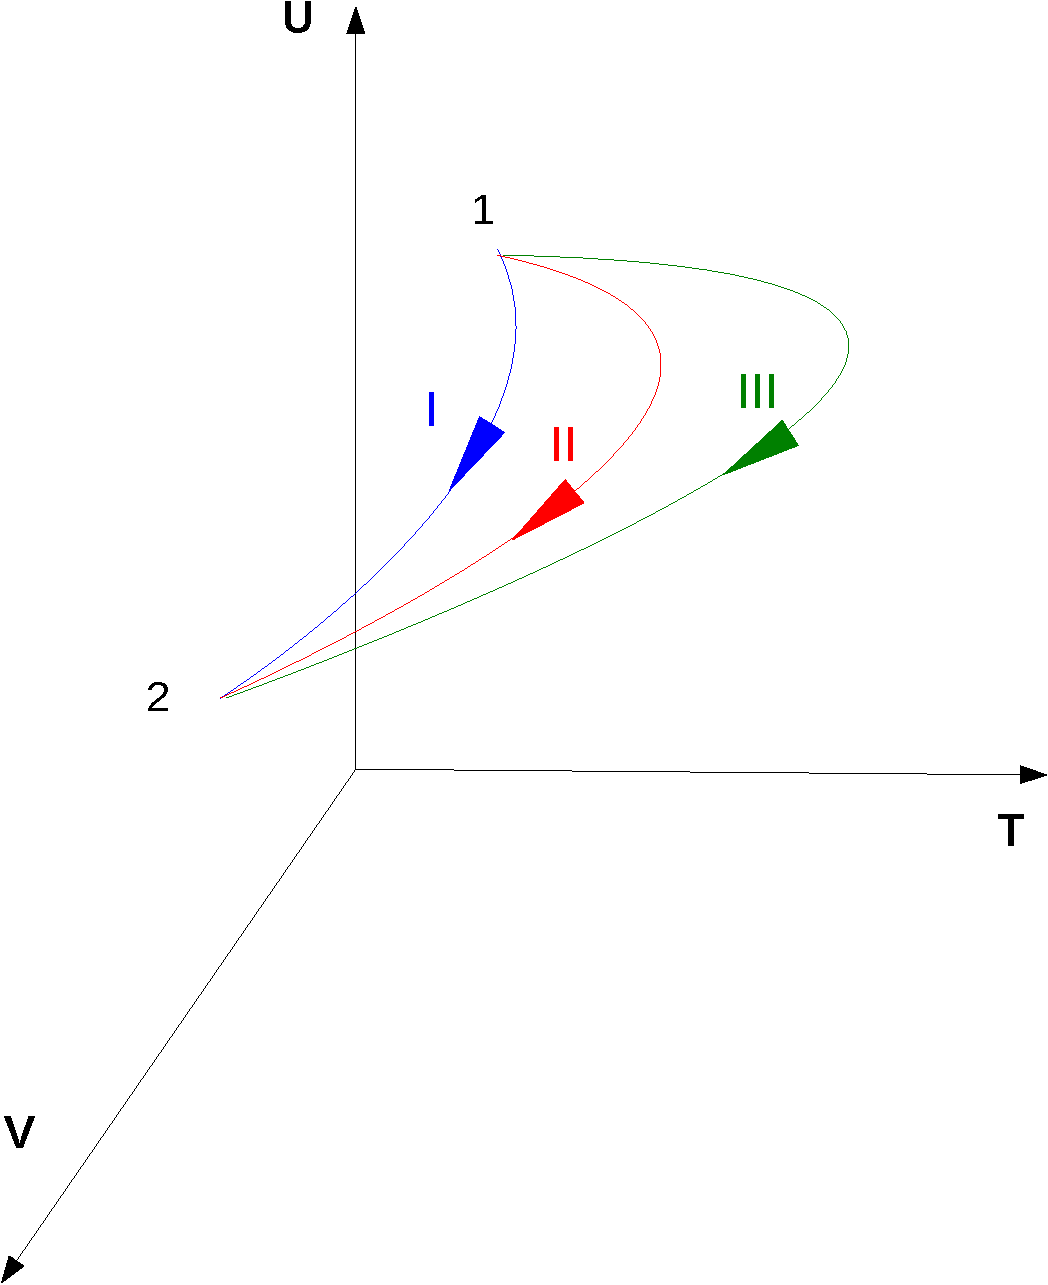
\includegraphics[width=9cm, height=9cm]{./Figs/Chp3_State-PathFunctions}
        \caption{State function: Change of internal function as a result of work and heat being exerted into the system by 3 distinct paths. Note that regardless the chosen path (from state 1 to state 2), $U_{1}$ and $U_{2}$ remain the same, although the amount of heat (represented here by changes in temperature, $T$) and work (\ie changes in volume, $V$) may vary significantly.}\label{Chapter:FirstLaw:Fig:StateFunctions}
     \end{center}
   \end{figure}
   
%%%
%%% SECTION
%%%
   \section{Reversible and Irreversible Processes}\label{Chapter:FirstLaw:Section:Reversibility}\index{Process!Reversible}\index{Process!Irreversible}
   Thermodynamic processes may change the state in two distinct ways:
   \begin{itemize}
     \item {\bf Reversible process} (also known as quasi-static process) is a process which can be stopped at any stage and reversed so that the system and the surroundings are exactly restored to their original states;
     \item {\bf Irreversible process} is a process in which heat is transferred through a finite temperature, thus it is not possible to return both the system and the surroundings to their original states.
   \end{itemize}
   Irreversibilities are of two types:
   \begin{itemize}
      \item {\it external irreversibilities} which are associated with dissipating effects outside the working fluid, \eg mechanical friction during a process due to some external force;
      \item {\it internal irreversibilities} which are associated with dissipating effects within the working fluid, \eg viscosity and inertial of a gas.
   \end{itemize}
   A set of definitions, characteristics and examples of these two processes are given by Table~\ref{Chapter:FirstLaw:TableDiffRevIrrev}. 
   
   
%%%
%%% SECTION
%%%
     \section{The First Law of Thermodynamics}\label{Chapter:FirstLaw:Section:FirstLaw}\index{Laws of Thermodynamics ! First law}
     \begin{subequations}
         Thermal energy is a macro-scale representation of micro-scale changes in mechanical energy (\ie work and heat). In a molecular scale, atoms and molecules are in random motion that can be associated with the kinetic energy of these `particles'. Tracking the motion and energy of each particle is addressed by a field of science called statistical (or quantum) thermodynamics; here we are interested in the consequences of the particles' motion, \ie oscillations in temperature as a measure of the average molecular-scale kinetic energy.
         \begin{shaded}
            \begin{center} {\bf Sign Notation}\end{center} 
              Before we proceed stating the {\it First Law}, we should define a sign notation used for all quantities in this document. Thus any form of energy:
              \begin{itemize}
                  \item Added to the system is assumed \blue{positive}, and;
                  \item Removed from the system is assumed \red{negative}.
              \end{itemize}
              Hence:
              \begin{itemize}
                 \renewcommand{\labelitemi}{$\star$}
                 \item heat added to the system by the neighbourhood is \blue{positive};
                 \item heat removed from the system to the neighbourhood is \red{negative};
                 \item work produced by the system and transferred to the neighbourhood is \red{negative};
                 \item work produced by the neighbourhood and transferred to the system is \blue{positive}.
              \end{itemize}
         \end{shaded}
         In most thermodynamic systems, changes in kinetic and potential energies are often assumed negligible\footnote{Here, we are assuming that such systems are not movable \wrt frames of reference.}, and Eqn.~\ref{Chapter:FirstLaw:Eqn:TotalEnergy3} becomes
            \begin{equation}
               \mfr[E]{2}{cv} - \mfr[E]{1}{cv} = U_{2}-U_{1} = Q_{1-2} + W_{1-2},\label{Chapter:FirstLaw:Eqn:FirstLaw1}
            \end{equation}
         in such cases, the internal energy of a system may be changed in any of the following ways: producing or receiving work and/or have heat being removed or added to the system. Heat and work are equivalent ways of changing the system's internal energy. It was experimentally observed that in isolated systems there is {\bf no} change in the internal energy.

         \begin{shaded}
            The {\it First Law of Thermodynamics} is effectively a statement of energy conservation: `the only way the energy of a closed system can be changed are through transfer of energy by work or heat' \citep{Moran_Book}. In other words: `the internal energy of an isolated system is constant' \citep{Atkins_Book}. Mathematically, these statements can be readily represented in differential form (\ie during infinitesimal changes in the state of the system) by,
            \begin{equation}
               d U = \delta Q + \delta W,\label{Chapter:FirstLaw:Eqn:FirstLaw2}
            \end{equation}
            
         \end{shaded}
   
     \end{subequations}

   %%%
   %%%
   \begin{landscape}
     \begin{table}
       \begin{tabular}{||l | l||}
         \hline\hline
             {\bf Reversible process} (RP)                                    &         {\bf Irreversible process}  (IP)                          \\
         \hline
             (a) RP can not be realised in practice;                          &  (a) All practical processes occurring are IP;                    \\
             (b) The process can be carried out in the reverse direction      &  (b) The process if carries out in reverse direction, it follows  \\
                 following the same path as followed in forward direction;    &      the path different from that in forward direction;           \\
             (c) A RP leaves no trace of occurrence of process upon the       &  (c) The evidences of process having occurred are evident even    \\
                 the system and surroundings after its reversal;              &      after reversal of IP;                                        \\
             (d) Such processes can occur in either directions without        &  (d) Occurrence of IPs in either directions is not possible, as   \\
                 violating the Second Law of Thermodynamics;                  &      in one direction it shall be accompanied with the violation  \\
                                                                              &      of the Second Law of Thermodynamics;                         \\
             (e) A system undergoing RPs has maximum efficiency. Therefore,   &  (e) Systems undergoing IPs do not have maximum efficiency as it  \\
                 sytems with RPs are considered as reference systems (\ie     &      accompanied by waste of energy;                              \\
                 benchmarks);                                                 &                                                                   \\
             (f) RPs occur at infinitesimal rate, \ie quasi-static process;   &  (f) IP occur at finite rate;                                     \\
             (g) System remains in thermodynamic equilibrium during occurrence&  (g) Systems does not remain in thermodynamic equilibrium during  \\
                 of such processes;                                           &      IPs;                                                         \\
         \hline
                                 {\bf Examples}                               &             {\bf Examples}                                        \\
             (h) Frictionless motion, controlled expansion and compression,   &   (h) Viscous fluid flow, inelastic deformation and hysteresis    \\
                 elastic deformations, polytropic expansion and compression   &       effects, free expansion, throttling processes, heat transfer\\
                 of fluids, electrolysis etc.                                 &       combustion, free expansion, diffusion etc.                  \\
         \hline\hline
       \end{tabular}
       \caption{Differences between reversible and irreversible processes \citep[extracted from][]{Singh_Book}.}
       \label{Chapter:FirstLaw:TableDiffRevIrrev}
     \end{table}
   \end{landscape}  
   
   % Example
   \begin{MyExample}{\begin{center}{\bf Example}\end{center}}
     \begin{example}\label{Chapter:FirstLaw:Example1}\citep{Atkins_Book}
        In a power station, the water pump is located in an isolated room. The electric motor of this pump produces 15 kJ of energy as mechanical work and loose 2 kJ of heat to the surroundings. Calculate the change in internal energy of the motor.  
     \end{example}

% SOLUTION
       \noindent{\bf Solution:}
       Here, the system is the electrical motor whereas the surroundings is the room. The work produced by the motor is $\delta W= -15$ kJ and the heat transferred from the engine to the room is $\delta Q = -2$ kJ, therefore 
          \begin{eqnarray}
             dU = \Delta U &=&  \delta Q + \delta W \nonumber \\
                &=& -15 -2 = -17\text{ kJ} \nonumber
          \end{eqnarray}
   \end{MyExample}

   % Example
   \begin{MyExample}{\begin{center}{\bf Example}\end{center}}
     \begin{example}\label{Chapter:FirstLaw:Example2}
       If $P_{1}$ = 3.00 atm, $V_{1}$ = 500 cm$^{3}$, $P_{2}$ = 1.00 atm and $V_{2}$ = 2000 cm$^{3}$. Calculate the work, $W_{\text{rev}}$ (in $J$), for the expansion processes shown in the following figure.
         \begin{center}
           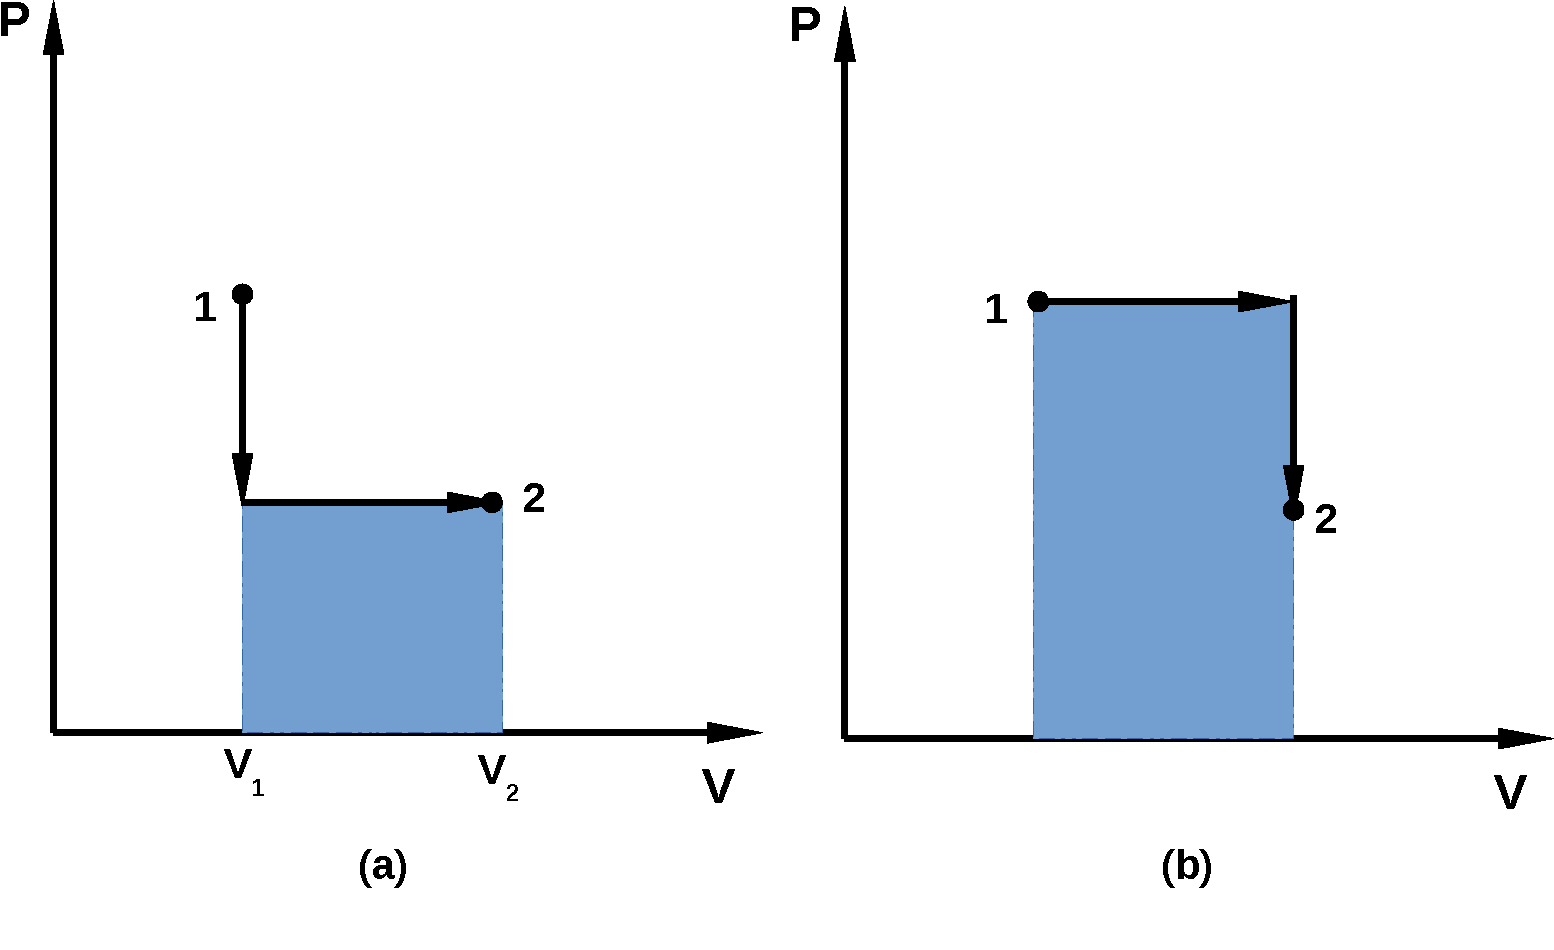
\includegraphics[width=.6\columnwidth,clip]{./Figs/Mod1Ex1}
         \end{center}
     \end{example}
     
% SOLUTION
       \noindent{\bf Solution:} $W_{\text{rev}}$ is related to the area below the curve. Thus, we should use the $PV$ work equation:
           \begin{itemize}
              \item For process {\bf (a)}: 
                 \begin{eqnarray}
                    d W = -PdV \Longrightarrow W &=& -P_{2}\left(V_{2}-V_{1}\right) \nonumber \\
                                                 &=& - 1\text{ atm}\left(2000-500\right)\text{ cm}^{3} = -1500\text{ atm.cm}^{3} \nonumber 
                 \end{eqnarray}
                 Now we need to convert {\it atm.cm}$^{3}$ to $J$, thus using the unit conversion table:
                 \begin{eqnarray}
                     W &=& -1500\blue{\cancel{\text{ atm}}}.\red{\cancel{\text{cm}^{3}}} \frc{1.01325\times 10^{5}\blue{\cancel{\text{ Pa}}}}{1\blue{\cancel{\text{ atm}}}} \frc{1 \frc{\text{kg}}{\text{m.s}^{2}}}{1\blue{\cancel{\text{ Pa}}}} \frc{1\text{ m}^{3}}{ 100^{3} \red{\cancel{\text{ cm}^{3}}}} \nonumber \\
                       &=& -151.9875 \blue{\cancel{\frc{\text{ kg.m}^{2}}{\text{s}^{2}}}} \frc{ 1 \text{ J}}{ \blue{\cancel{\frc{\text{ kg.m}^{2}}{\text{s}^{2}}}}} \nonumber\\
                       &=& -151.9875\text{ J} \nonumber
                 \end{eqnarray}
%
              \item For process {\bf (b)}, since $P$ is constant, i.e., $P_{1}=P_{2}$:
                 \begin{eqnarray}
                    d W = -PdV \Longrightarrow W &=& -P_{1}\left(V_{2}-V_{1}\right) \nonumber \\
                                                 &=& - 3\text{ atm}\left(2000-500\right)\text{ cm}^{3} = -4500\text{ atm.cm}^{3} \nonumber \\
                                                 &=& -455.9625\text{ J} \nonumber
                 \end{eqnarray}
           \end{itemize}
   \end{MyExample}

%%%
%%% SECTION
%%%
     \section{Cycles: Representation of the First Law}\label{Chapter:FirstLaw:Section:FirstLaw_Cycle}\index{Laws of Thermodynamics ! First law}\index{Cycles}
        \begin{subequations}
           \begin{shaded}
               During any cycle, the cyclic integral of heat added to a system is proportional to the cyclic integral of work done by the system.
           \end{shaded}
           This statement clearly indicates that during a cycle the internal energy is zero, $\left(\Delta U\right)_{\text{cycle}}=0$. The mathematical representation of the first law in a cycle is
             \begin{equation}
               \displaystyle\oint \delta Q = -\displaystyle\oint \delta W,\label{Chapter:FirstLaw:Eqn:FirstLawCycle}
             \end{equation}
             where line integral $\left(\oint\right)$ is defined in Appendix~\ref{Appendix_Calculus:Section:LineIntegral}. Two main practical systems arise from the application of the first law to the definition of cycles (Section~\ref{Chapter:Introduction:Section:Introduction:ProcessesCyclesDefinition}): power and refrigeration cycles.
      
%%%% SUBSECTION
          \subsection{Power Cycles}\index{Cycles! Power }
             Power cycles (Fig.~\ref{Chapter:FirstLaw:Fig:PowerRefrigSystems}a) are systems that deliver a net work transfer of energy to the surroundings during each cycle, where
               \begin{displaymath}
                  W_{cycle} = Q_{in} - Q_{out},\;\;\;\text{ with }\;\;\; Q_{in} > Q_{out}.
               \end{displaymath}
             The energy supplied by heat transfer to a system on a power cycle is often derived from combustion processes. Such cycles are used to quantitatively describe the work produced in power plants, and are often assessed through the thermal efficiency of the process,\index{Cycles! Power! Thermal efficiency }
       \begin{equation}
           \eta =\frc{W_{cycle}}{Q_{in}} = \frc{Q_{in} - Q_{out}}{Q_{in}} = 1 - \frc{Q_{out}}{Q_{in}} < 1.\label{Chapter:FirstLaw:Eqn:FirstLawCycle:PowerEfficiency}
       \end{equation}
       For reversible power cycles the ratio of heat transfer, $Q_{cold}/Q_{hot}$ depends only on the reservoirs' temperatures and can be simplified to
       \begin{equation}
          \frc{Q_{\text{cold}}}{Q_{\text{hot}}} =  \frc{T_{\text{cold}}}{T_{\text{hot}}}.\label{Chapter:FirstLaw:Eqn:FirstLawCycle:PowerEfficiency2}
       \end{equation}
       One of the conditions for this expression to be valid is $T_{\text{hot}}\ne0$, indeed {\bf reservoir temperature are always assumed as absolute temperature, \ie expressed in Kelvin}.
       \begin{shaded}
           Thus the thermal efficiency of a reversible power cycle while operating between thermal reservoirs at temperatures $T_{hot}$ and $T_{cold}$ is expressed as
          \begin{equation}
            \eta_{\text{max}} = 1 - \frc{T_{\text{cold}}}{T_{\text{hot}}}\label{Chapter:FirstLaw:Eqn:FirstLawCycle:PowerCarnotEfficiency}
          \end{equation}
          $\eta_{\text{max}}$ is also known as the {\it Carnot efficiency}\index{Carnot Efficiency} and it is the maximum efficiency any power cycle can have while operating between the 2 reservoirs.
       \end{shaded}

   \begin{figure}[h]
      \vbox{
        \hbox{ \hspace{-1.5cm}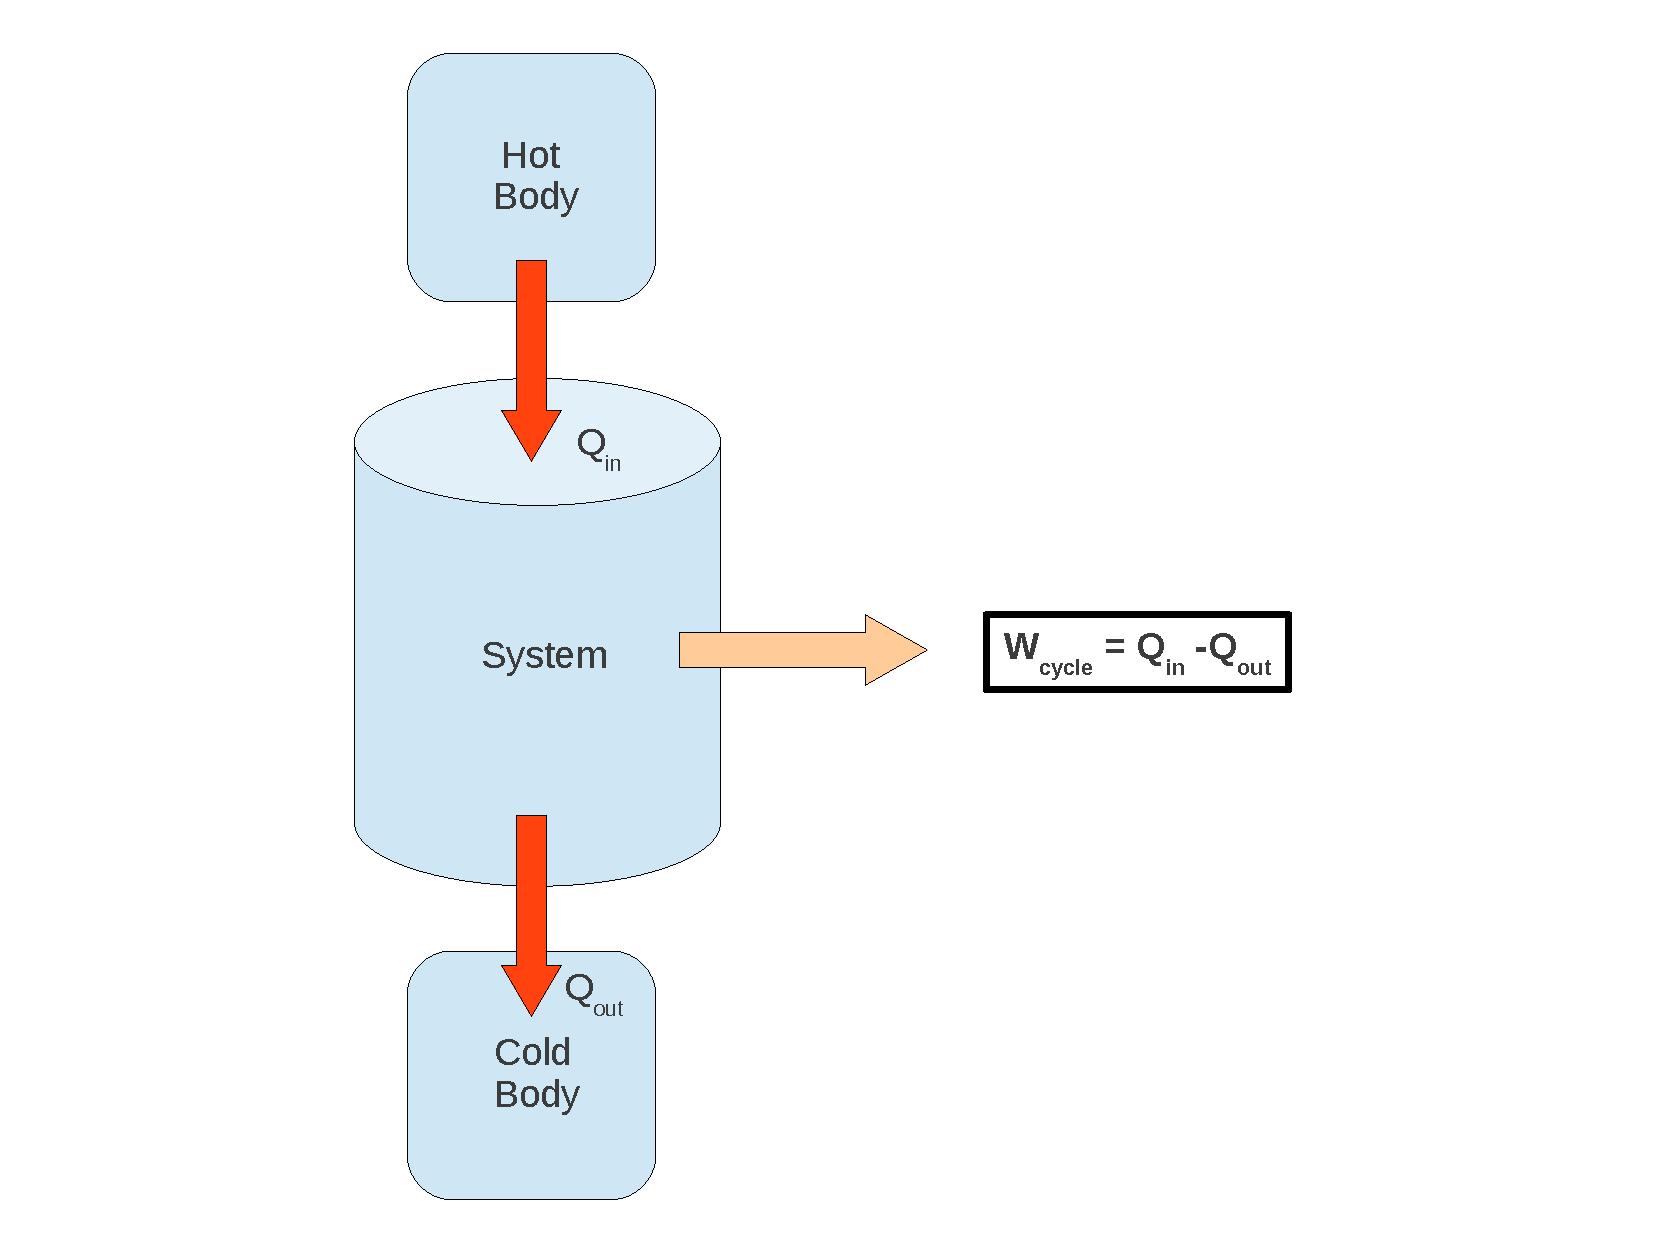
\includegraphics[width=.7\columnwidth,clip]{./Figs/FirstLaw_Cycle_01}
               \hspace{-2.5cm}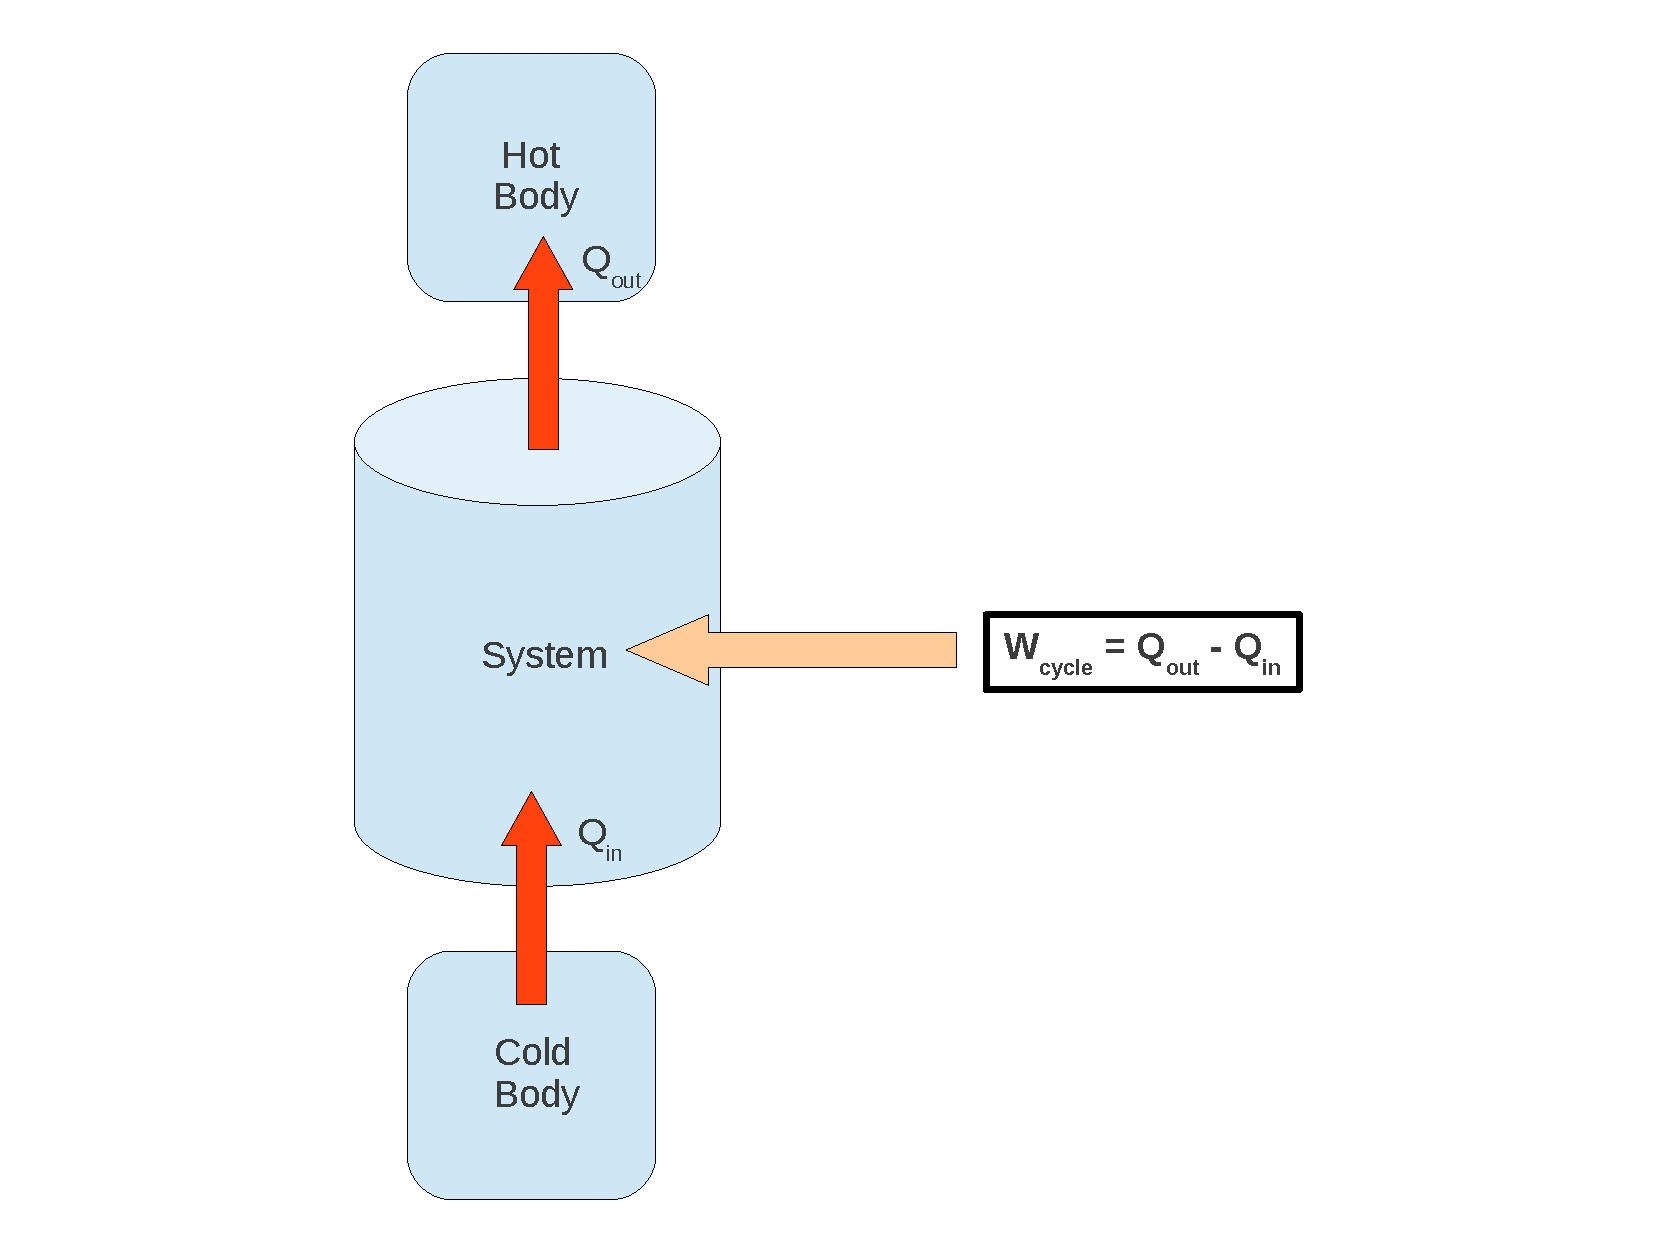
\includegraphics[width=.7\columnwidth,clip]{./Figs/FirstLaw_Cycle_02}}
        \vspace{-0.cm}
        \hbox{\hspace{4cm}(a)\hspace{7cm}(b)}}
       \caption{Schematic representation of (a) power and (b) refrigeration cycles.}\label{Chapter:FirstLaw:Fig:PowerRefrigSystems}
   \end{figure}    

%%%% SUBSECTION
          \subsection{Refrigeration Cycles}\index{Cycles! Refrigeration }
           Refrigeration cycles (Fig.~\ref{Chapter:FirstLaw:Fig:PowerRefrigSystems}b) are systems in which Q$_{in}$ is associated with the heat energy transferred into the system from the cold body. Q$_{out}$ is the energy discharged via heat transfer from the system to the hot body, 
           \begin{displaymath}
              W_{cycle} = Q_{out} - Q_{in}.
           \end{displaymath}
            \begin{shaded}
               The aim of such cycles is to cool a refrigerated body or to maintain the temperature of a body bellow that of the surrounding. Refrigeration cycles are assessed through the coefficient of performance (COP)\index{Cycles!Refrigeration ! Coefficient of performance },
                 \begin{equation}
                   \beta = \frc{Q_{in}}{W_{cycle}} = \frc{Q_{in}}{Q_{out} - Q_{in}}.\label{Chapter:FirstLaw:Eqn:FirstLawCycle:COP}
                 \end{equation}
          \end{shaded}
        \end{subequations}
   

%%%
%%% SECTION
%%%
     \section{Enthalpy}\label{Chapter:FirstLaw:Section:Enthalpy}\index{Enthalpy}
        \begin{subequations}
          Let's consider a gas contained in a piston-cylinder system undergoing a quasi-static isobaric process. Let's also assume that there are no changes in kinetic and potential energies and that the only work done during the process is the one associated with the piston's movement. The first law stated that the internal energy is a result of changes in work and heat,
          \begin{displaymath}
            dU = \delta Q + \delta W,\;\;\;\text{ and } \;\;\; \delta W = -\int\limits_{1}^{2} PdV = -P\left(V_{2}-V_{1}\right).
          \end{displaymath}
          \begin{shaded}
             Replacing the work into the first law equation
             \begin{eqnarray}
                \delta Q &=& dU - \delta W = U_{2} - U_{1} + P_{2}V_{2} - P_{1}V_{1}\nonumber \\
                         &=& \left(U_{2}+P_{2}V_{2}\right) - \left(U_{1}+P_{1}V_{1}\right).\label{Chapter:FirstLaw:Eqn:EnthalpyDefinition1}
             \end{eqnarray}
             The terms in brackets, $U+PV$, are thermodynamic properties that depend only on the state of the system and, as such, define a new extensive property, the {\it enthalpy},
             \begin{equation}
               H\equiv U + PV.\label{Chapter:FirstLaw:Eqn:EnthalpyDefinition2}
             \end{equation}
             Replacing Eqn.~\ref{Chapter:FirstLaw:Eqn:EnthalpyDefinition1} in \ref{Chapter:FirstLaw:Eqn:EnthalpyDefinition2}
             \begin{equation}
               \delta Q = \overbrace{\left(U_{2}+P_{2}V_{2}\right)}^{H_{2}} - \overbrace{\left(U_{1}+P_{1}V_{1}\right)}^{H_{1}} = H_{2}-H_{1} = \Delta H,\label{Chapter:FirstLaw:Eqn:EnthalpyDefinition3}
             \end{equation}
             \ie the {\it change in enthalpy leads to the heat transfer for isobaric processes}. 
          \end{shaded}
       
        \end{subequations}

%%%
%%% SECTION
%%%
    \section{Heat Capacities}\label{Chapter:FirstLaw:Section:HeatCapacity}
      \begin{subequations}

        %%% Subsection
        \subsection{Constant Volume and Constant Pressure Heat Capacities}\index{Heat Capacity ! Constant Volume}\index{Heat Capacity ! Constant Pressure}\index{$C_{v}$| see{ Heat Capacity}}\index{$C_{p}$| see{ Heat Capacity}}
            {\it Specific heat capacity} can be defined as the amount of heat necessary to increase the temperature of a unit mass of material by one degree. Mathematically, it can be defined as
            \begin{displaymath}
              C\equiv \frc{1}{m}\frc{\delta Q}{\delta T}.
            \end{displaymath}
            As $Q$ is path-dependent, $C$ also is, and from the first law
            \begin{displaymath}
              \delta Q = dU - \delta W \;\;\Longrightarrow\;\; dU + PdV,
            \end{displaymath}
            two properties can be defined depending upon the path:
            \begin{enumerate}[(i)]
              \item Constant volume: in which the term $PdV$ vanishes and the specific heat at constant volume $\left(C_{v}\right)$ is
                \begin{equation}
                  C_{v} = \frc{1}{m}\left(\frc{\delta Q}{\delta T}\right)_{V} = \frc{1}{m}\left(\frc{\partial U}{\partial T}\right)_{V} = \left(\frc{\partial u}{\partial T}\right)_{V}\label{Chapter:FirstLaw:Eqn:HeatCapacityConstVolume1}
                \end{equation}
              \item Constant pressure: in which the work term can be integrated at constant pressure, hence the heat transfer can be expressed in terms of the enthalpy change (Eqn.~\ref{Chapter:FirstLaw:Eqn:EnthalpyDefinition3}),
                \begin{equation}
                  C_{p} = \frc{1}{m}\left(\frc{\delta Q}{\delta T}\right)_{P} = \frc{1}{m}\left(\frc{\partial H}{\partial T}\right)_{P} = \left(\frc{\partial h}{\partial T}\right)_{P}\label{Chapter:FirstLaw:Eqn:HeatCapacityConstPressure1}
                \end{equation}
            \end{enumerate}
            $C_{p}\left(T,P\right)$ and $C_{v}\left(T,v\right)$ are thermodynamic properties for general materials and can vary with the independent variables $\left(T, P, v\right)$. Here, $h$ and $u$ are specific enthalpy and internal energy with units J.kg$^{-1}$.
            
        %%% Subsection
        \subsection{Heat Capacity Relations for Ideal Gases}\label{Chapter:FirstLaw:Section:HeatCapacity:IdealGas}
          For ideal gases, one can use the fundamental thermodynamic relation that defined enthalpy (Eqn.~\ref{Chapter:FirstLaw:Eqn:EnthalpyDefinition2}) and the ideal gas EOS, $Pv=RT$ (Eqn.~\ref{Chapter:Intro_Property_of_Gases:Eqn:IdealEOS}), to redefine the specific enthalpy
          \begin{equation}
            h = u(T) + RT,\label{Chapter:FirstLaw:Eqn:EnthalpyDefinition4}
          \end{equation}
          of an ideal gas as a function of $T$ only, \ie $h=h(T)$.  The specific heat of an ideal gas at contant volume is expressed as
          \begin{displaymath}
             C_{v}(T,v) = \left(\frc{\partial u}{\partial T}\right)_{v} = \frc{d}{dT}\left(u(T)\right) = C_{v}(T).
          \end{displaymath}
          In other words, $C_{v}$ is property that can be expressed as function of $T$ and $v$ (thus being defined as a partial differential equation with the differential operator $\partial$), however if a process is assumed isochoric (\ie constant volume) this property becomes a function of only the temperature (and therefore defined as an ordinary differential equation with the differential operator $d$),
                \begin{equation}
                  du = C_{v}(T)dT.\label{Chapter:FirstLaw:Eqn:HeatCapacityConstVolume2}
                \end{equation}
          A similar argument can be used for $C_{p}$ in isobaric processes, leading to
                \begin{equation}
                  dh = C_{p}(T)dT.\label{Chapter:FirstLaw:Eqn:HeatCapacityConstPressure2}
                \end{equation}
          \begin{shaded}
             Differentiating Eqn.~\ref{Chapter:FirstLaw:Eqn:EnthalpyDefinition4} and replacing $du$ and $dh$,
                \begin{eqnarray}
                   && dh = du + RdT \nonumber \\
                   && C_{p}(T)dT = C_{v}(T)dT + RdT \;\;\;\Longrightarrow C_{p}(T) = C_{v} + R \nonumber \\
                   && C_{p}(T) - C_{v}(T) = R.\label{Chapter:FirstLaw:Eqn:HeatCapacitiesRelation_IdealGas1}
                \end{eqnarray}
             A useful relationship in engineering thermodynamics is the ratio of specific heats (or isentropic index),
                \begin{equation}
                  \gamma = \frc{C_{p}}{C_{v}},\label{Chapter:FirstLaw:Eqn:HeatCapacitiesRelation1}
                \end{equation}
             which is valid for any material. For an ideal gas, this relation reduces to 
                \begin{equation}
                  \gamma = \frc{C_{v}(T)+R}{C_{v}(T)} = 1 + \frc{R}{C_{v}(T)}.\label{Chapter:FirstLaw:Eqn:HeatCapacitiesRelation_IdealGas2}
                \end{equation}
             Other heat capacity based relations for ideal gases can be obtained from Eqns.~\ref{Chapter:FirstLaw:Eqn:FirstLaw2}, \ref{Chapter:FirstLaw:Eqn:EnthalpyDefinition2} and \ref{Chapter:Intro_Property_of_Gases:Eqn:IdealEOS}:
                \begin{equation}
                   \delta Q = 
                      \begin{cases}
                         C_{p}dT - \frc{RT}{P}dP, \label{Chapter:FirstLaw:Eqn:HeatCapacitiesRelation_IdealGas3} \\
                         \frc{C_{p}}{R}PdV + \frc{C_{v}}{R}VdP.
                      \end{cases}
                \end{equation}
                These relations, although apparently simple, reveal the dependence of heat transfer on temperature, pressure and volume in processes involving ideal gases.
          \end{shaded}


        \end{subequations}


   % Example
   \begin{MyExample}{\begin{center}{\bf Example}\end{center}}
     \begin{example}\label{Chapter:FirstLaw:Example3}
       Calculate the internal energy (in $J$) when 1 mol of water is isobarically heated from 25$^{\circ}$C to 30$^{\circ}$C at 1 atm. Given: densities of water are 0.9970 g.cm$^{-3}$ at 0$^{\circ}$C and 0.9956 g.cm$^{-3}$ at 100$^{\circ}$C. Molar mass and heat capacity at constant pressure of water are 18 g.mol$^{-1}$ and 1 cal.$\left(\text{g.}^{\circ}\text{C}\right)^{-1}$, respectively.
     \end{example}
     
% SOLUTION
       \noindent{\bf Solution:} From the 1$^{\text{st}}$ Law, $U=Q+W$ ,and in order to calculate $U$ we first need to obtain heat ($Q$) and work ($W$). $Q$ can be obtained from the heat capacity equation
          \begin{displaymath}
             Q = m C_{p} \Delta T,
          \end{displaymath}  
          where $m$ is the mass of water can be obtained from
          \begin{displaymath}
             n = \frc{m}{MW} \Longrightarrow  m = n.MW = 1\text{ mol} . 18 \frc{\text{g}}{\text{mol}} = 18 \text{ g}
          \end{displaymath}
          $n$ and $MW$ are number of moles and molar mass, respectively. Now,
          \begin{displaymath}
             Q = m C_{p} \Delta T = 18\text{ g} . 1 \frc{\text{ cal}}{\text{g.}^{\circ}\text{C}}.\left(30-25\right)^{\circ}\text{C} = 90\text{ cal}
          \end{displaymath}  
          Now, we should calculate the work through $W=-P\Delta V$, however $V$ is not known, but we can obtain it from the density relation $V=m/\rho$, thus
          \begin{displaymath}
             W = - P\Delta V = -P\left(V_{2}-V_{1}\right) = -P\left(\frc{m}{\rho_{2}} - \frc{m}{\rho_{1}}\right) = -0.025\text{atm.cm}^{3} = -0.0006\text{ cal} 
          \end{displaymath}
          Now, calculating the internal energy,
          \begin{displaymath}
             U = Q + W = 89.9994\cancel{\text{ cal}} . \frc{ 4.186\text{ J}}{1\cancel{\text{ cal}}} = 376.7375 \text{ J}
          \end{displaymath}
   \end{MyExample}


   % Example
   \begin{MyExample}{\begin{center}{\bf Example}\end{center}}
     \begin{example}\label{Chapter:FirstLaw:Example4}\citep{Rajput_Book}
       A 0.3 m$^{3}$  tank contains oxygen initially at 100 kPa and 300 K. A paddle wheel within the tank is rotated until the pressure inside rise to 150 kPa. During the process 2 kJ of heat is lost to the surroundings. Determine the paddle-wheel work done (in kJ). Neglect the energy stored in the paddle wheel and assume the heat capacity at constant volume of oxygen is 0.6745 kJ.$\left(\text{kg.K}\right)^{1}$. Given molar mass of oxygen of 32 g.mol$^{-1}$.
     \end{example}
     
% SOLUTION
       \noindent{\bf Solution:} The volume of the tank remains constant $V_{2}=V_{1}=V=$ 0.3 m$^{3}$ during the whole process. Thus, we can define:
            \begin{center}
              \begin{tabular}{l l l l}
                 Initial Condition & $P_{1}=$ 100 kPa   & $T_{1}=$ 300 K         & $V_{1}=$ 0.3 m$^{3}$  \\
                 Final Condition   & $P_{2}=$ 150 kPa   &                       & $V_{2}=$ 0.3 m$^{3}$ \\
                 Heat Loss         & $Q=$ -2 kJ        &                       &                    
              \end{tabular}
            \end{center}
       The compression occurs in a closed system (i.e., constant mass) and, as there is no further information, we may consider that oxygen behaves as an ideal gas. The work added to the system by the paddle can be expressed by $U=Q+W$. Our first step is to calculate $T_{2}$,
       \begin{displaymath}
          \frc{P V}{T} = \text{ constant} \Rightarrow \frc{P_{1}V_{1}}{T_{1}} = \frc{P_{2}V_{2}}{T_{2}} \Rightarrow \frc{P_{1}}{T_{1}}=\frc{P_{2}}{T_{2}} \Rightarrow T_{2} = 450\text{ K}
       \end{displaymath}
        The specific internal energy can defined by the fundamental relation, $du=C_{v}dT$ (check the units for this relation!), where $C_{v}$ is the heat capacity at constant volume thus,
       \begin{displaymath}
          \Delta U = m\Delta u = C_{v}\Delta T = Q + W,
       \end{displaymath}
       therefore, we need to obtain the mass of oxygen in the tank through the ideal gas equation of state,
       \begin{eqnarray}
         P V = n R T \Rightarrow n = \frc{m}{MW} = \frc{P V}{R T} \Rightarrow m &=& \frc{ MW P V}{R T} \nonumber \\
                                                      &=& \frc{ 32\frc{\text{ g}}{\text{mol}} 100\text{ kPa} . 0.3\text{ m}^{3}}{ 8.3143 \frc{\text{J}}{\text{mol.K}} 300\text{ K}} \nonumber \\
                                                      &=& 0.3848 \frc{\text{ g.kPa.m}^{3}}{\text{J}} \frc{1 \text{ J}}{1\text{ N.m}} \frc{1000 \text{ Pa}}{1 \text{ kPa}} \frc{ 1 \text{ N.m}^{-2}}{1\text{ Pa}} \nonumber\\
                                                      &=& 0.3848\text{ kg}\nonumber
       \end{eqnarray}
       Thus
       \begin{eqnarray}
          \Delta u = m C_{v}\Delta T = Q + W \Rightarrow W &=& m C_{v}\left(T_{2}-T_{1}\right) - Q \nonumber \\
                                                          &=& 0.3848\text{ kg} \times 0.6745 \frc{\text{kJ}}{\text{kg.K}}\times (450-300)\text{ K} - (-2 \text{ kJ}) \nonumber \\
                                                          &=& 40.9321\text{ kJ}. \nonumber
       \end{eqnarray}
       The paddle-wheel executed 40.9321 kJ of work to the system.
   \end{MyExample}
   
   % Example
   \begin{MyExample}{\begin{center}{\bf Example}\end{center}}
     \begin{example}\label{Chapter:FirstLaw:Example4}\citep{Atkins_Book}
       Calculate the change in molar enthalpy of N $_{2}$(g) when it is heated from 25$^{\circ}$C to 100$^{\circ}$C. The heat capacity is given by
       \begin{displaymath}
         C_{p} = a + bT + \frc{c}{T^{2}}, 
       \end{displaymath}
       where $\left[C_{p}\right]=$ J.mol$^{-1}$.K$^{-1}$, $\left[T\right]=$ K, $a=$ = 28.58 J.mol$^{-1}$.K$^{-1}$, $b=$ 3.77$\times$10$^{-3}$ J.mol$^{-1}$ and $c=$ -0.50$\times$10$^{5}$ J.mol$^{-1}$.K. Given molar enthalpy of N $_{2}$(g) at 25$^{\circ}$C is 29.1400 J.mol$^{-1}$.
     \end{example}
     
% SOLUTION
     \noindent{\bf Solution:} As all units contain temperature in Kelvin, let's first convert them as $T_{1}=$ 298.15 K and $T_{2}=$ 373.15 K. Now, we need to calculate the change in molar enthalpy in this temperature range using the definition of heat capacity,
        \begin{eqnarray}
          && C_{p} = \left(\frc{\partial H}{\partial T}\right)_{P} \;\;\Longrightarrow\;\; dH = C_{p}dT \nonumber \\
          && \int\limits_{H_{1}\left(T_{1}\right)}^{H_{2}\left(T_{2}\right)}dH = \int\limits_{T_{1}}^{T_{2}} C_{p}dT = \int\limits_{T_{1}}^{T_{2}} \left(a + bT + \frc{c}{T^{2}}\right)dT \nonumber \\
          && H_{2}\left(T_{2}\right) - H_{1}\left(T_{1}\right) = a\left(T_{2}-T_{1}\right) + \frc{1}{2}b\left(T_{2}^{2}-T_{1}^{2}\right) - c\left(\frc{1}{T_{2}}-\frc{1}{T_{1}}\right) \nonumber 
        \end{eqnarray}
        Solving this expression with the constants and $H_{1}\left(T_{1}\right)=H\left(\text{298.15 K}\right)=$ 29.14 J.mol$^{-1}$, leads to $H_{2}\left(T_{2}\right) = H\left(\text{373.15 K}\right)=$ 2238.4047 J.mol$^{-1}$. Thus, change in molar enthalpy, \ie $H_{2}\left(T_{2}\right) - H_{1}\left(T_{1}\right)$,  of N $_{2}$(g) is 2209.2647 J.mol$^{-1}$.

   \end{MyExample} 
       
      
%%%
%%% SECTION
%%%
     \section{Work Done at Moving Boundary}\label{Chapter:FirstLaw:Section:Work}
     \begin{subequations}
        In Section~\ref{Chapter:Introduction:Section:ThermodynamicWorkHeat}, the work produced by (or exerted on) the system was defined by Eqn.~\ref{Chpt01_Work2},
           \begin{equation}
              dW = -PdV \;\;\Longrightarrow \;\; W = - \int\limits_{V_{1}}^{V_{2}} PdV,\label{Chapter:FirstLaw:Eqn:Work1}
           \end{equation}
        where $P$ is the pressure and $V$ is the variable volume. Let's consider a system comprising a cylinder containing a compressible gas $\left(\text{with }V_{1}\text{ and } P_{g} = P_{1}\right)$ with a movable piston (Fig.~\ref{Chapter:FirstLaw:Fig:Work1}). An external pressure $\left(P_{\text{ext}} > P_{1}\right)$ is imposed on the piston and continuously compress the gas until the pressures are equalised $\left(P_{\text{ext}} = P_{g} = P_{2}\right)$. At the end of such compression (\ie at state 2) $V_{2}<V_{1}$ and the work $W$ is positive, \ie energy is transferred to the system through the application of an external force. Now, let's assume that at state 2, $P_{\text{ext}}$ is replaced by a new pressure, $P^{\star}_{\text{ext}}=P_{1}$, such that $P^{\star}_{\text{ext}} < P_{\text{ext}} \left(= P_{g} = P_{2}\right)$. As the new pressure is smaller than the pressure inside the cylinder $\left(P_{2}\right)$, the gas will expand until the external and internal pressure are equal, \ie $P_{g} = P^{\star}_{\text{ext}} = P_{1}$. At the end of such expansion from $V_{2}$ to $V_{1}$, the work
           \begin{displaymath}
              W = - \int\limits_{V_{2}}^{V_{1}} PdV,
           \end{displaymath}
           is negative, \ie energy is transferred from the system to the neighbourhood. In these expansion and compression processes, two scenarios may occur: constant or variable pressures. Equation~\ref{Chapter:FirstLaw:Eqn:Work1} is solved according with these scenarios.
\medskip
% Figure
   \begin{figure}[h]
     \begin{center}
        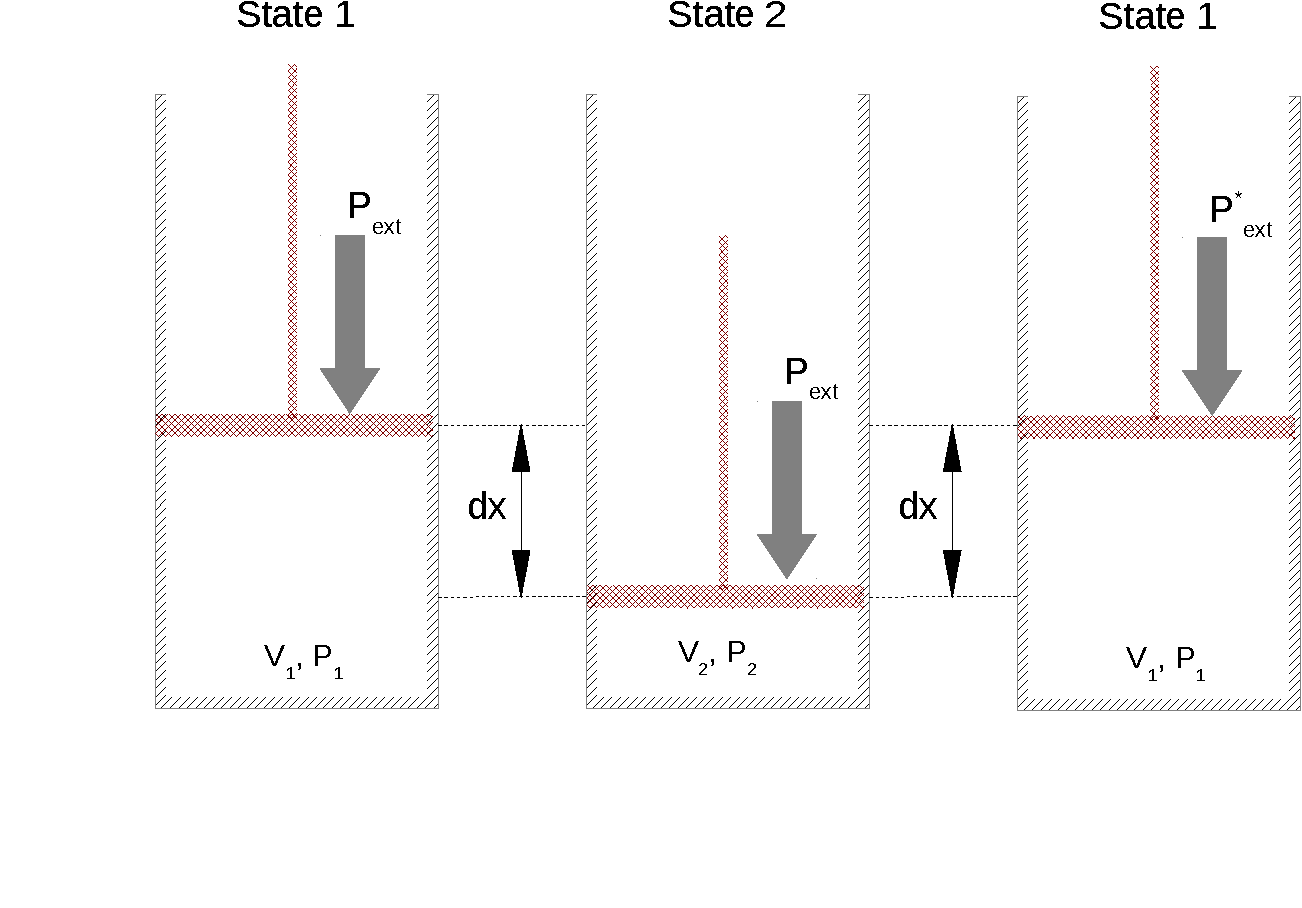
\includegraphics[width=0.7\columnwidth,clip]{./Figs/Chp3_PistonCylinder1}\vspace{-2cm}
        \caption{Compression and expansion of a piston as a result of an external force.}\label{Chapter:FirstLaw:Fig:Work1}
     \end{center}
   \end{figure}
\medskip


%%%
%%% SECTION
%%%
     \subsection{Expansion/Compression under Constant Pressure}\label{Chapter:FirstLaw:Section:Work_ConstantPressure}
        If the external pressure $P=P_{\text{ext}}$ is constant, the integral (Eqn.~\ref{Chapter:FirstLaw:Eqn:Work1}) can be readily solved with the initial and final volumes,
           \begin{shaded}
             \begin{equation}
                dW = -PdV \;\;\Longrightarrow \;\; W = - P\int\limits_{V_{1}}^{V_{2}} dV = - P\left(V_{2}-V_{1}\right) = -P\Delta V.\label{Chapter:FirstLaw:Eqn:Work_ConstPressure}
             \end{equation}
           \end{shaded}
           This integral can be graphically illustrated by the area under the $PV$ curve of Fig.~\ref{Chapter:FirstLaw:Fig:Work2}a. The work is equal to area beneath the horizontal line at $P=P_{\text{ext}}$ lying between $V_{1}$ and $V_{2}$.
           
% Figure
\begin{figure}[h]
  \vbox{
     \hbox{\hspace{2cm}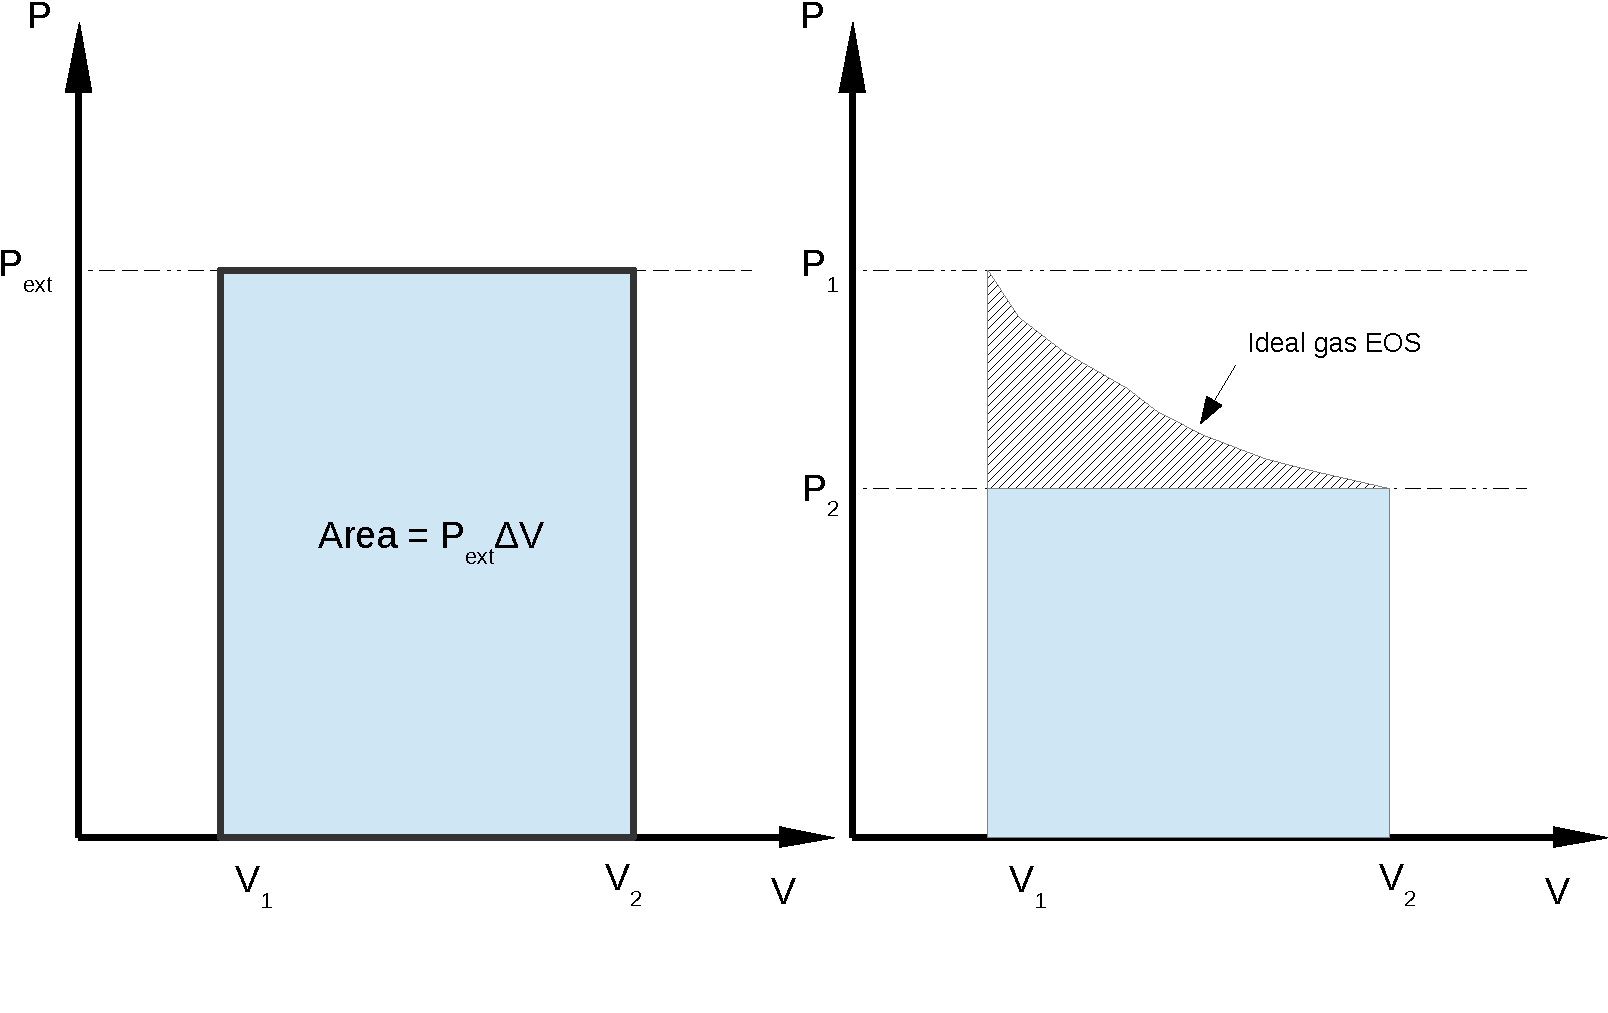
\includegraphics[width=0.7\columnwidth,clip]{./Figs/Chp3_PistonCylinder2}}
     \vspace{-1.cm}
     \hbox{\hspace{5cm}(a)\hspace{4.5cm}(b)}}%\vspace{-0.cm}
        \caption{Ideal gas expansion under isothermal conditions: (a) irreversible work at constant external pressure is equal to the blue area (Eqn.~\ref{Chapter:FirstLaw:Eqn:Work_ConstPressure}); (b) reversible work from $V_{1}$ to $V_{2}$ is given by the area below the curve (\ie blue and hatched areas).}\label{Chapter:FirstLaw:Fig:Work2}
   \end{figure}

%%%
%%% SECTION
%%%
     \subsection{Reversible Expansion}\label{Chapter:FirstLaw:Section:Work_ReversibleExpansion}
     In reversible processes, changes in the state can be reversed by infinitesimal modification of relevant properties. Let's suppose a gas confined in the piston-cylinder system (Fig.~\ref{Chapter:FirstLaw:Fig:Work1}) at stage 2. If the external pressure, $P_{\text{ext}}$ is set equal to the gas pressure, $P_{2}$, thus there is no movement of the piston as the system is in mechanical equilibrium with the surroundings. Any infinitesimal change in $P_{\text{ext}}$ leads to changes in volume, \ie an infinitesimal reduction in the external pressure results in slight expansion of the gas (increase of the volume), whereas an infinitesimal increase of the external pressure leads to slight gas contraction (decrease of the volume).

     In both scenarios, the change is reversible, however if the external pressure differs measurably from the internal (gas) pressure, then changing $P_{\text{ext}}$ infinitesimally will not change the volume of the gas (\ie the direction of the piston movement). Such a system is not in mechanical equilibrium with its surroundings and the expansion/contraction is thermodynamically irreversible.

     For reversible expansion, $P_{\text{ext}}$ is assumed to be equal to $P$ (internal gas pressure) at each stage of the expansion, $P_{\text{ext}}=P$,
           \begin{shaded}
             \begin{equation}
                dW_{\text{rev}} = -P_{\text{ext}}dV = -PdV \;\;\Longrightarrow \;\; W_{\text{rev}} = -\int\limits_{V_{1}}^{V_{2}}PdV.\label{Chapter:FirstLaw:Eqn:Work_ReversibleExpansion}
             \end{equation}
             The integral can only be evaluated once the behaviour of the confined pressure is known and can be expressed by an algebraic equation as a function of the volume.
           \end{shaded}

           \begin{MyBlock}{Isothermal Reversible Expansion}
             Let's suppose a scenario in which an ideal gas undergoes an isothermal reversible expansion. In such scenario, the system (\eg piston-cylinder) remains in thermal equilibrium with its surrounding at a prescribed and constant temperature (\eg a constant temperature bath). In this case, $T$, $R$ and $n$ (closed system) are constants and may be taken outside the integral (Eqn.~\ref{Chapter:FirstLaw:Eqn:Work_ReversibleExpansion}), and the integral from $V_{1}$ to $V_{2}$ becomes,
             \begin{equation}
               W_{\text{rev}} = -\int\limits_{V_{1}}^{V_{2}}PdV = -n R T\int\limits_{V_{1}}^{V_{2}}\frc{dV}{V} = -n R T\ln{\frc{V_{2}}{V_{1}}}.\label{Chapter:FirstLaw:Eqn:Work_IsothermalReversibleExpansion}
             \end{equation}
             If the final volume is larger than the initial volume $\left(V_{2} > V_{1}\right)$ (as in any expansion), the logarithm term in Eqn.~\ref{Chapter:FirstLaw:Eqn:Work_IsothermalReversibleExpansion} is positive, thus $W_{\text{rev}}$ is negative, \ie, the system has produced work. Similarly, if the gas undergoes a compression $\left(\text{and therefore } V_{2} < V_{1}\right)$, thus $W_{\text{rev}}$ is positive as the logarithm term is negative.

             The work produced during the isothermal reversible expansion of an ideal gas is graphically represented in Fig.~\ref{Chapter:FirstLaw:Fig:Work2}b. Reversible work (integral $PdV$) is the (blue + hatched) area under the ideal gas EOS curve from $V_{1}$ to $V_{2}$, whereas the area in blue is effectively the irreversible work at a constant external pressure $P_{\text{ext}} = P_{2}$. Such graphical representation shows that reversible work is larger than the corresponding irreversible work of a similar system.
           \end{MyBlock}


   % Example
   \begin{MyExample}{\begin{center}{\bf Example}\end{center}}
     \begin{example}\label{Chapter:FirstLaw:Example6}\citep{Rajput_Book}
       A gas contained in a piston-cylinder system undergoes a reversible compression from 1.5 to 7.5 bar. The gas behaves according to the following expression
       \begin{displaymath}
         PV = C,
       \end{displaymath}
       where [$P$] and [$V$] are in bar and m$^{3}$, respectively, and $C$ = 3 bar.m$^{3}$ Calculate the work (in kJ) done during the compression.
     \end{example}

% SOLUTION
       \noindent{\bf Solution:} For a reversible compression from $P_{1}$ = 1.5 to $P_{2}$ = 7.5 bar to happen, work needs to be given to the system and can be calculated from
         \begin{displaymath}
           W_{\text{rev}} = -\int\limits_{V_{1}}^{V_{2}}PdV
         \end{displaymath}
       As the gas behaves according to the relation, $V=\frac{3}{P}$, we can readily conclude that initial and final volumes are 2.00 and 0.40 m$^{3}$, respectively. Now, integrating from $V_{1}$ to $V_{2}$ and replacing $P$ with $\frac{3}{V}$,
         \begin{displaymath}
           W_{\text{rev}} = -\int\limits_{V_{1}}^{V_{2}}PdV = - \int\limits_{V_{1}}^{V_{2}} \frc{C}{V}dV = -C\int\limits_{V_{1}}^{V_{2}} \frc{dV}{V} = -C \ln{\frc{V_{2}}{V_{1}}} = 4.8283\text{ bar.m}^{3} = 482.83\text{ kJ}.
         \end{displaymath}
         As the product of the logarithm term has {\bf no units}, the unit of the work is the same as $C$, \ie bar.m$^{3}$. Also, note that the work is positive, therefore the transfer of energy as work occurs from the surroundings to the piston-cylinder system.
   \end{MyExample}


   % Example
   \begin{MyExample}{\begin{center}{\bf Example}\end{center}}
     \begin{example}\label{Chapter:FirstLaw:Example7}\citep{Rajput_Book}
       A fluid at pressure of 3 bar and with specific volume of 0.18 m$^{3}.\text{kg}^{-1}$ is allocated in a piston-cylinder system and expands reversibly to 0.6 bar according to an experimental relation, $P = Cv^{-2}$, where $C$ is a constant and $v$ is the specific volume. Calculate the work $\left(\text{in kJ.kg}^{-1}\right)$ done by the fluid on the piston.
     \end{example}

% SOLUTION
       \noindent{\bf Solution:} The work from the reversible process can be obtained by integrating Eqn.~\ref{Chapter:FirstLaw:Eqn:Work_ReversibleExpansion} from $v_{1}$ to $v_{2}$,
         \begin{displaymath}
           W_{\text{rev}} = -\int\limits_{v_{1}}^{v_{2}}Pdv = -\int\limits_{v_{1}}^{v_{2}}\frc{C}{v^{2}}dv = -C\int\limits_{v_{1}}^{v_{2}}\frc{dv}{v^{2}} = -C\left.\left(-\frc{1}{v}\right)\right|_{v_{1}}^{v_{2}}
         \end{displaymath}
      Note that in this example we are integrating based on the specific volume ($v$) instead of the total volume ($V$). Such change of volume-based property does not alter the expression for work, we just need to make sure that all calculations are conducted in a consistent way throughout the problem. In order to solve this expression, we also need to calculate the fluid volume after the expansion, $v_{2}$, and the constant $C$.

     We can calculate both unknowns through the given experimental relation,
         \begin{eqnarray}
           && C = P_{1}v_{1}^{2} = 0.0972\text{ bar.m}^{6}\text{.kg}^{-2} \nonumber \\
           && P_{1}v_{1}^{2} = C = P_{2}v_{2}^{2}\;\; \Longrightarrow \;\; v_{2} = 0.4025\text{ m}^{3}\text{.kg}^{-1} \nonumber
         \end{eqnarray}
     Now, solving the integral with $v_{2}$ and $C$,
         \begin{eqnarray}
           W_{\text{rev}} &=& -\int\limits_{v_{1}}^{v_{2}}Pdv = -C\left.\left(-\frc{1}{v}\right)\right|_{v_{1}}^{v_{2}} = -C\left(-\frc{1}{v_{2}}+\frc{1}{v_{1}}\right) = -2.9851\times 10^{-1}\text{ bar.m}^{3}\text{.kg}^{-1} \nonumber \\
                       &=& -29.8510\text{ kJ}\text{.kg}^{-1} \nonumber
         \end{eqnarray}
         As indicated by the sign, the work is produced by the system and exerted into the surroundings.
   \end{MyExample}
     \end{subequations}
   
%%%
%%% SECTION
%%%
   \section{Polytropic Processes}\label{Chapter:FirstLaw:Section:PolytropicProcesses}\index{Process!Polytropic}
   In the previous sections, the path-dependence of the work added or produced -- $W=-\int PdV$, was a result of the different ways to compress/expand fluids, represented by the area under a curve in a $PV$ diagram (Fig.~\ref{Chapter:FirstLaw:Fig:Work_PV}). The area under the curve defined by path $A$ is clearly different from the one defined under the curve of path $B$, in fact
   \begin{displaymath}
     W_{12}^{A} > W_{12}^{B},
   \end{displaymath}
   as the work depends on the path selected, and not only on the initial and final coordinates. Several real thermodynamics processes are often described by {\it polytropic processes} in which,
   \begin{equation}
     PV^{n} = \text{constant} = C, \hspace{.5cm} \text{ with }\label{Chapter:FirstLaw:Eqn:PolytropicProcess}
     \begin{cases}
       n = 0,  & \text{ isobaric;}\\
       n = 1, & \text{ isothermal (for ideal gases);} \\
       0 < n < 1 \text{ or } 1 < n < \infty, & \text{ polytropic;} \\
       n = \gamma = \frc{C_{p}}{C_{v}}, & \text{ adiabatic (\ie isentropic) process;}\\
       n = \infty, & \text{ isochoric.}
     \end{cases}
   \end{equation}
   where $n$ is the (positive) polytropic exponent.
   
% Figure
\begin{figure}[h]
  \vbox{
     \hbox{\hspace{2cm}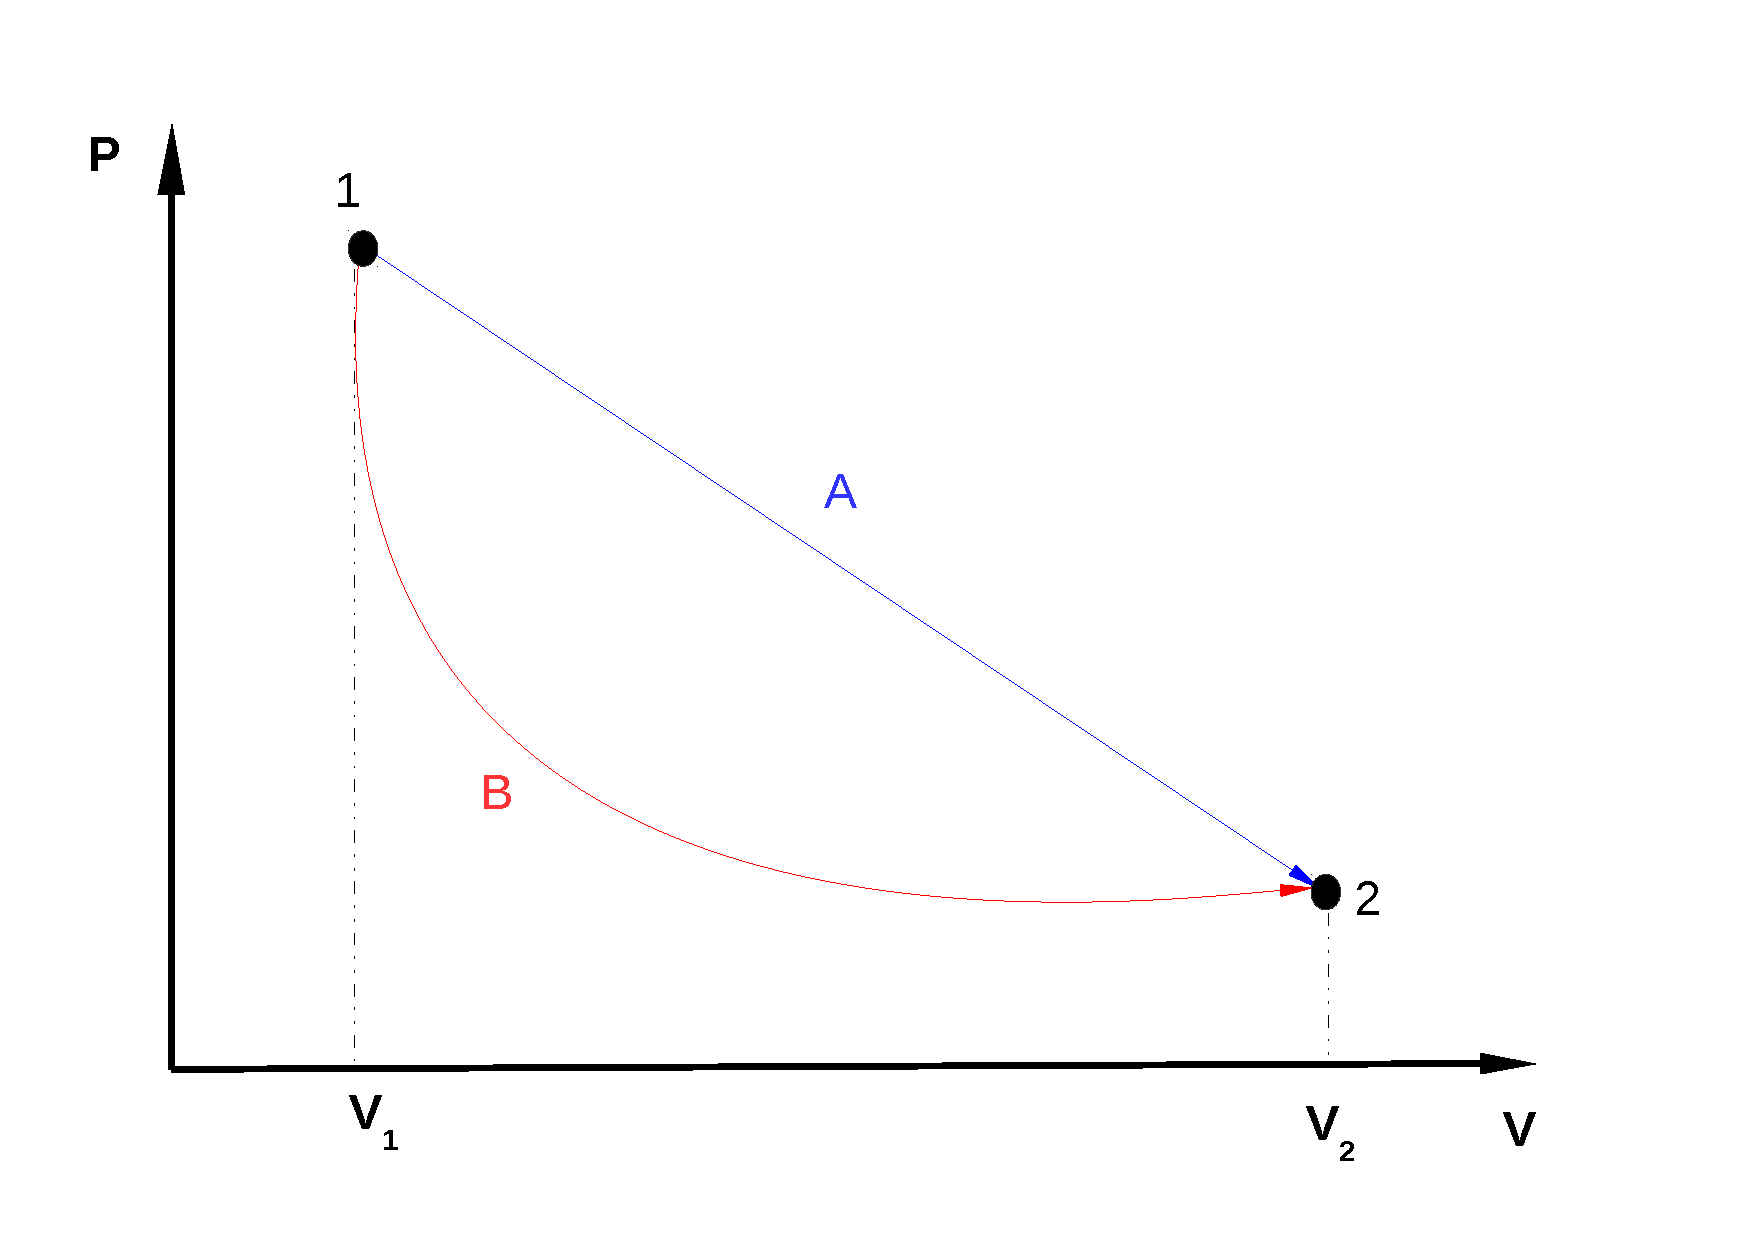
\includegraphics[width=0.7\columnwidth,clip]{./Figs/Chp3_PistonCylinder_PV}}}
        \caption{Gas expansion under different conditions represented by 2 paths.}\label{Chapter:FirstLaw:Fig:Work_PV}
   \end{figure}

   
%%%
%%% SECTION
%%%
   \section{Reversible Adiabatic Processes}\label{Chapter:FirstLaw:Section:ReversibleAdiabaticProcesses}\index{Process!Adiabatic}
     \begin{subequations}

       A process is named {\it adiabatic} when no heat is transferred to or from the system (\ie $\delta Q$ = 0),
         \begin{equation}
           dU = \cancelto{0}{\delta Q} + \delta W \;\;\Longrightarrow\;\; \Delta U = U_{2}-U_{1}= W.
         \end{equation}
       This equation is valid for both reversible and irreversible processes\index{Process!Reversible}\index{Process!Irreversible}, and can only be ensured if a perfect thermal insulation is achieved.  For mechanically reversible adiabatic (\ie isentropic) compression / expansion of ideal gases,
      \begin{eqnarray}
          dU &=& \delta Q + \delta W \;\;\Longrightarrow \;\; \delta Q = C_{v}dT + PdV = 0 \nonumber \\
          dT &=& -\frc{P}{C_{v}}dV  \;\; \left(\text{Constraint: } C_{v}\ne 0\right) \nonumber \\
             &=& -\frc{RT}{V C_{v}}dV \;\; \Rightarrow \;\; \frc{dT}{T} = - \frc{R}{C_{v}}\frc{dV}{V}. \label{Chapter:FirstLaw:Eqn:AdiabaticProcesses1}
      \end{eqnarray}
      Integrating Eqn.~\ref{Chapter:FirstLaw:Eqn:AdiabaticProcesses1} and assuming $C_{v}$ is constant,
           \begin{eqnarray}
              &&\int\limits_{T_{1}}^{T_{2}} \frc{dT}{T} = \frc{R}{C_{v}}\int\limits_{V_{1}}^{V_{2}}\frc{dV}{V} \;\;\Longrightarrow\;\;  \left.\ln{T}\right|_{T_{1}}^{T_{2}} = \left.-\frc{R}{C_{v}}\ln{V}\right|_{V_{1}}^{V_{2}}\nonumber \\
              &&\ln{\frc{T_{2}}{T_{1}}} = -\frc{R}{C_{v}}\ln{\frc{V_{2}}{V_{1}}} = \ln{\left(\frc{V_{1}}{V_{2}}\right)^{\frac{R}{C_{v}}}}\;\;\Longrightarrow\;\; \frc{T_{2}}{T_{1}} = \left(\frc{V_{1}}{V_{2}}\right)^{\frac{R}{C_{v}}} \nonumber
           \end{eqnarray}
           Now, using the ratio of specific heats defined in Eqn.~\ref{Chapter:FirstLaw:Eqn:HeatCapacitiesRelation_IdealGas2}, 
           \begin{displaymath}
              \gamma = 1 + \frc{R}{C_{v}},
           \end{displaymath}
           in the previous relation,
           \begin{shaded}
             \begin{equation}
                TV^{\gamma-1} = \text{ constant}\label{Chapter:FirstLaw:Eqn:AdiabaticProcesses_TVGamma}
             \end{equation}
           \end{shaded}

           Now from Eqn.~\ref{Chapter:FirstLaw:Eqn:HeatCapacitiesRelation_IdealGas3},
           \begin{displaymath}
               \delta Q = C_{p}dT - \frc{RT}{P}dP = 0,
           \end{displaymath}
           and assuming $C_{p}$ is constant and different from zero,
           \begin{eqnarray}
             && \int\limits_{T_{1}}^{T_{2}}\frc{dT}{T} = \frc{R}{C_{p}}\int\limits_{P_{1}}^{P_{2}}\frc{dP}{P} \;\;\Longrightarrow\;\; \left.\ln{T}\right|_{T_{1}}^{T_{2}} = \left.\frc{R}{C_{p}} \ln{P}\right|_{P_{1}}^{P_{2}} \nonumber \\
             && \ln{\frc{T_{2}}{T_{1}}} = \ln{\left(\frc{P_{2}}{P_{1}}\right)^{\frac{R}{C_{p}}}} \;\;\Longrightarrow\;\;  \frc{T_{2}}{T_{1}} = \left(\frc{P_{2}}{P_{1}}\right)^{\frac{R}{C_{p}}}.\nonumber
           \end{eqnarray}
           Again, using  Eqn.~\ref{Chapter:FirstLaw:Eqn:HeatCapacitiesRelation_IdealGas2},
           \begin{shaded}
             \begin{equation}
                TP^{\frac{1-\gamma}{\gamma}} = \text{ constant}\label{Chapter:FirstLaw:Eqn:AdiabaticProcesses_TPGamma}
             \end{equation}
           \end{shaded}
           
           Finally, integrating the right-hand side from Eqn.~\ref{Chapter:FirstLaw:Eqn:HeatCapacitiesRelation_IdealGas3},
           \begin{eqnarray}
               && \delta Q = \frc{C_{v}}{R}VdP + \frc{C_{p}}{R}PdV = 0 \;\; \Longrightarrow \;\; \frc{C_{v}}{\cancel{R}}VdP = -\frc{C_{p}}{\cancel{R}}PdV \;\;\Longrightarrow\;\; C_{v}\int\limits_{P_{1}}^{P_{2}} \frc{dP}{P} = -C_{p}\int\limits_{V_{1}}^{V_{2}}\frc{dV}{V} \nonumber \\
              && \left.\ln{P}\right|_{P_{1}}^{P_{2}} = -\left.\frc{C_{p}}{C_{v}}\ln{V}\right|_{V_{1}}^{V_{2}} \;\; \Longrightarrow \;\;\frc{P_{2}}{P_{1}} = \left(\frc{V_{1}}{V_{2}}\right)^{\frac{C_{p}}{C_{v}}}\nonumber 
           \end{eqnarray}
           Again, using  Eqn.~\ref{Chapter:FirstLaw:Eqn:HeatCapacitiesRelation_IdealGas2},
           \begin{shaded}
             \begin{equation}
                PV^{\gamma} = \text{ constant}\label{Chapter:FirstLaw:Eqn:AdiabaticProcesses_PVGamma}
             \end{equation}
           \end{shaded}
     \end{subequations}



   % Example
   \begin{MyExample}{\begin{center}{\bf Example}\end{center}}
     \begin{example}\label{Chapter:FirstLaw:Example8}\citep{Rajput_Book}
       Air initially occupying 1 m$^{3}$ at 1.5 bar and 20$^{\circ}$C undergoes an internally reversible compression for which $P V^{\gamma}=$ constant to a final state where the pressure is 6 bar and the temperature is 120$^{\circ}$C. Determine:
        \begin{enumerate}[(a)]
           \item Value of $\gamma$;
           \item Work and the heat transfer (in kJ).
       \end{enumerate}
       Assume that heat capacity at constant volume and molar mass of air are 0.718 kJ.$\left(\text{kg.K}\right)^{-1}$ and 29 g.mol$^{-1}$.
     \end{example}

% SOLUTION
       \noindent{\bf Solution:} 
        \begin{center}
           \begin{tabular}{c c c c}
               {\bf State}  &   $P$ (atm)  &   $T\;\left(^{\circ}\text{C}\right)$ & $V\;\left(\text{m}^{3}\right)$ \\
                    1       &     1.5      &            20                      & 1  \\
                    2       &     6.0      &            120                     &     \\              
           \end{tabular}
        \end{center}
        \begin{enumerate}[(a)]
           \item In order to calculate the isentropic index $\gamma$, we can use any of the relations learned in the lecture,
               \begin{displaymath} 
                   P V^{\gamma} = C, \hspace{1cm} T V^{\gamma-1} = C \hspace{1cm} \text{ and/or } \hspace{1cm} T P^{\frac{1-\gamma}{\gamma}} = C.
               \end{displaymath}
               Although $P$ and $V$ is the relation initially given in the problem, we do not know the final volume of air, $V_{2}$. However, initial and final pressure and temperature are known and we can make use of this relationship to obtain $\gamma$,
               \begin{eqnarray} 
                   T P^{\frac{1-\gamma}{\gamma}} = C \Rightarrow T_{1}P_{1}^{\frac{1-\gamma}{\gamma}} = T_{2}P_{2}^{\frac{1-\gamma}{\gamma}} \nonumber \\
                   \left(\frc{P_{1}}{P_{2}}\right)^{\frac{1-\gamma}{\gamma}} = \frc{T_{2}}{T_{1}} \Rightarrow \frc{1-\gamma}{\gamma} = \frc{\ln{\frac{T_{2}}{T_{1}}}}{\ln{\frac{P_{1}}{P_{2}}}} \Longrightarrow \gamma = 1.2686  \nonumber
               \end{eqnarray}
                 
           \item Compression work can be obtained by integrating $\d W = -P dV$ from state 1 to state 2 with $P=\frac{C}{V^{\gamma}}$,
               \begin{eqnarray}
                 W_{1-2} &=& -\int\limits_{V_{1}}^{V_{2}} P dV = -\int\limits_{V_{1}}^{V_{2}}\frc{C}{V^{\gamma}} dV = -\left.\frc{C}{1-\gamma}V^{1-\gamma}\right|_{V_{1}}^{V_{2}} \nonumber \\
                         &=& -\frc{C}{1-\gamma}\left(V_{2}^{1-\gamma}-V_{1}^{1-\gamma}\right),\;\;\text{ however, as } C=P_{1}V_{1}^{\gamma}=P_{2}V_{2}^{\gamma} \nonumber \\
                         &=& -\frc{P_{2}V_{2}^{\gamma}V_{2}^{1-\gamma} - P_{1}V_{1}^{\gamma}V_{1}^{1-\gamma}}{1-\gamma} = \frc{P_{1}V_{1}-P_{2}V_{2}}{1-\gamma} \nonumber
               \end{eqnarray}
               The relation above, although important, can not be used as we do not know $V_{2}$, however we can change variables through the ideal gas relation
               \begin{eqnarray}
                 P V = n R T &\Rightarrow& n = \frc{P V}{R T } = \frc{1.5\text{ atm} \times 1\text{ m}^{3}}{ 8.3143 \frc{\text{J}}{\text{mol.K}} 293.15\text{ K}} \frc{1.01325\times 10^{5} \text{ Pa}}{1 \text{ atm}} \frc{ 1 \text{ N.m}^{-2}}{1\text{ Pa}}\frc{1 \text{ J}}{1\text{ N.m}} \nonumber \\
                 &&  n = 62.3580\text{ moles} \nonumber \\
                   % m &=& \frc{P_{1} V_{1} MW}{R T_{1}} = \frc{1.5\text{ atm} \times 1\text{ m}^{3} \times 29 \frac{\text{g}}{\text{mol}} } { 8.3143 \frc{\text{J}}{\text{mol.K}} 293.15\text{ K}} \frc{1 \text{ J}}{1\text{ N.m}} \frc{1.01325\times 10^{5} \text{ Pa}}{1 \text{ atm}} \frc{ 1 \text{ N.m}^{-2}}{1\text{ Pa}} = 1808.38 \text{ g}\nonumber\\
                    W &=& \frc{P_{1}V_{1}-P_{2}V_{2}}{1-\gamma} = nR\frc{T_{1}- T_{2}}{1-\gamma} \nonumber \\
                      &=& 62.3580\text{ mol} \times 8.3143 \frc{\text{J}}{\text{mol.K}} \times \frc{\left(293.15-393.15\right)\text{ K}}{1-1.2686} \nonumber \\
                      &=& 193024.2440 \text{ J} \Longrightarrow W = -193.02 \text{ kJ} \nonumber
               \end{eqnarray}
              Heat ($Q$) can be obtained from
               \begin{eqnarray}
          \Delta u &=& m C_{v}\Delta T = n MW C_{v}\Delta T = Q + W  \nonumber \\
             Q &=& n MW C_{v}\left(T_{2}-T_{1}\right) - W \nonumber \\
               &=& 62.3580\text{ mol}\times 29 \frc{\text{g}}{\text{mol}} \red{\frc{1\text{ kg}}{1000\text{ g}}}\times 0.718\frc{\text{kJ}}{\text{kg.K}}\times (393.15-293.15)\text{ K} - 193.30 \text{ kJ} \nonumber \\
                                                          &=& -63.46\text{ kJ}. \nonumber                   
               \end{eqnarray}
        \end{enumerate}
   \end{MyExample}
   

   
\clearpage   
\begin{FinalSummaryBlock}{Summary}
    \begin{itemize}
       \item Work is the transfer of energy by motion against an opposing force;
       \item Heat is the transfer of energy as a result of temperature differences between the system and the surroundings;
       \item Internal energy is the energy stored in the components of the system. The internal energy of an ideal gas is a function of temperature only;
       \item The First Law of thermodynamics states that heat and work are mutually convertible, however as energy can not be either created or destroyed, the internal energy associated with an energy conversion remains constant, $dU = \delta q + \delta w$;
       \item The energy of an isolated system is always constant;
       \item A reversible change is a change that can be reversed by an infinitesimal modification of a variable. Maximum work is achieved in a reversible change;
       \item The enthalpy is defined as $H = U + PV$. The enthalpy change is the energy transferred as heat at constant pressure, $\Delta H = Q$;
       \item Heat capacity at constant volume is defined as $C_{v}=\left(\partial U / \partial T\right)_{V}$. The heat capacity at constant pressure is defined as $C_{p}=\left(\partial H / \partial T\right)_{P}$;
       \item In case of:
         \begin{itemize}
            \item Reversible isochoric process (\ie $V=$ constant):
              \begin{displaymath}
                \Delta U = C_{v}\left(T_{2}-T_{1}\right), \;\; W = 0\;\; Q = C_{v}\left(T_{2}-T_{1}\right);
              \end{displaymath}
            \item Reversible isobaric process (\ie $P=$ constant):
              \begin{displaymath}
                \Delta U = C_{v}\left(T_{2}-T_{1}\right), \;\; W = P\left(V_{2}-V_{1}\right)\;\; Q = C_{p}\left(T_{2}-T_{1}\right);
              \end{displaymath}
            \item Reversible adiabatic process (\ie $PV^{\gamma}=$ constant):
              \begin{displaymath}
                 \frc{T_{2}}{T_{1}} = \left(\frc{V_{1}}{V_{2}}\right)^{\gamma-1} = \left(\frc{P_{2}}{P_{1}}\right)^{\frc{\gamma-1}{\gamma}};
              \end{displaymath}
            \item Polytropic reversible process (\ie $PV^{n}=$ constant):
              \begin{displaymath}
                 \frc{T_{2}}{T_{1}} = \left(\frc{V_{1}}{V_{2}}\right)^{n-1} = \left(\frc{P_{2}}{P_{1}}\right)^{\frc{n-1}{n}}.
              \end{displaymath}
         \end{itemize}
    \end{itemize}
\end{FinalSummaryBlock}
